\documentclass[12pt,a4paper]{article}

% -------------------------------------------------
% PACOTES
% -------------------------------------------------
\usepackage[utf8]{inputenc}
\usepackage[T1]{fontenc}
\usepackage[brazil]{babel}
\usepackage[a4paper,margin=2.5cm]{geometry}
\usepackage{graphicx}
\usepackage{float}
\usepackage{placeins}
\usepackage{fancyhdr}
\usepackage{lastpage}
\usepackage{titlesec}
\usepackage{booktabs}
\usepackage{longtable}
\usepackage{array}
\usepackage{hyperref}
\usepackage{xcolor}
\usepackage{enumitem}
\usepackage{setspace}
\usepackage{ragged2e}

\hypersetup{
    colorlinks=true,
    linkcolor=black,
    urlcolor=blue,
    citecolor=black,
    pdftitle={RFC - Request for Comments — Projeto de Portfólio}
}

\setlength{\parindent}{1.25cm}
\setlength{\parskip}{0.2cm}
\onehalfspacing

% -------------------------------------------------
% DADOS DO DOCUMENTO
% -------------------------------------------------
\newcommand{\logoarquivo}{Imagens/logo_catolica.png}
\newcommand{\instituicao}{Católica SC}
\newcommand{\turma}{T2ESOFT07NB}
\newcommand{\titulo}{RFC: Request for Comments — Projeto de Portfólio}
\newcommand{\curso}{Engenharia de Software}
\newcommand{\autor}{André Luiz Michels da Silva}
\newcommand{\orientador}{Diogo Vinícius Winck}
\newcommand{\dataentrega}{\today}

% -------------------------------------------------
% CABEÇALHO E RODAPÉ
% -------------------------------------------------
\pagestyle{fancy}
\fancyhf{}
\renewcommand{\headrulewidth}{0.4pt}
\renewcommand{\footrulewidth}{0.4pt}
\fancyhead[L]{Conteúdo}
\fancyhead[R]{%
  \IfFileExists{\logoarquivo}{\includegraphics[height=1.1cm]{\logoarquivo}}{\small \instituicao}%
}
\fancyfoot[L]{Turma:\hspace{0.5em}\turma}
\fancyfoot[C]{Instituição:\hspace{0.5em}\instituicao}
\fancyfoot[R]{Página:\hspace{0.5em}\thepage\ de \pageref{LastPage}}

% Página inicial sem cabeçalho/rodapé padrão
\fancypagestyle{plain}{
  \fancyhf{}
  \renewcommand{\headrulewidth}{0pt}
  \renewcommand{\footrulewidth}{0.4pt}
  \fancyfoot[L]{Turma:\hspace{0.5em}\turma}
  \fancyfoot[C]{Instituição:\hspace{0.5em}\instituicao}
  \fancyfoot[R]{Página:\hspace{0.5em}\thepage\ de \pageref{LastPage}}
}

% -------------------------------------------------
% FORMATAÇÃO DE TÍTULOS
% -------------------------------------------------
\titleformat{\section}
  {\normalfont\Large\bfseries}
  {\thesection.}
  {0.5em}
  {}

\titleformat{\subsection}
  {\normalfont\large\bfseries}
  {\thesubsection}
  {0.5em}
  {}

\titleformat{\subsubsection}
  {\normalfont\normalsize\bfseries}
  {\thesubsubsection}
  {0.5em}
  {}

% -------------------------------------------------
% COMANDOS AUXILIARES
% -------------------------------------------------
\providecommand{\rf}[2]{#1 & #2 \\\midrule}
\providecommand{\rnf}[2]{#1 & #2 \\\midrule}

\begin{document}

% -------------------------------------------------
% CAPA
% -------------------------------------------------
\begin{titlepage}
    \centering

    \vspace*{1.2cm}

    \IfFileExists{\logoarquivo}{\includegraphics[width=0.28\textwidth]{\logoarquivo}\par}{\vspace*{2cm}}

    \vspace{1.5cm}
    {\Large \instituicao\par}

    \vfill

    \noindent\rule{\textwidth}{0.4pt}
    \vspace{0.4cm}

    {\Huge \titulo\par}
    \vspace{0.45cm}
    {\Large \curso\par}

    \vspace{0.4cm}
    \noindent\rule{\textwidth}{0.4pt}

    \vfill

    {\Large \autor\par}

    \vspace{1.8cm}
    {\large Orientador: \orientador\par}

    \vfill

    {\large \dataentrega\par}
\end{titlepage}

% -------------------------------------------------
% SUMÁRIO
% -------------------------------------------------
\pagenumbering{roman}
\tableofcontents
\clearpage
\pagenumbering{arabic}

% -------------------------------------------------
% IDENTIFICAÇÃO
% -------------------------------------------------
\section*{Identificação}
\addcontentsline{toc}{section}{Identificação}

\begin{itemize}[leftmargin=1.5cm]
    \item \textbf{Título do Projeto:} Modelo de Análise Preditiva para Consumo de Insumos Hospitalares
    \item \textbf{Linha de Projeto (Direction):} Web / IA / Dados.
    \item \textbf{Autor:} André Luiz Michels da Silva.
    \item \textbf{Data da Proposta:} 05/03/2026.
    \item \textbf{Versão:} 1.0.
\end{itemize}

% -------------------------------------------------
\section{Visão do Produto e Impacto (O Problema)}

\subsection{Contexto e Problema}

No setor hospitalar, o gerenciamento de estoques e suprimentos representa um grande desafio devido à complexidade operacional envolvida e à grande diversidade de materiais e medicamentos utilizados diariamente. Em muitas instituições de saúde, os custos relacionados à cadeia de suprimentos podem representar entre 20\% e 46\% dos gastos operacionais do hospital, tornando a gestão eficiente desses recursos um fator crítico para a sustentabilidade financeira da instituição \cite{aptel2001, barbieri2006}.\\

\noindent{Além disso, a dificuldade em prever o consumo de determinados insumos pode resultar em dois problemas recorrentes: excesso de estoque, que pode levar ao desperdício de materiais por vencimento de validade, e falta de insumos essenciais, comprometendo a continuidade do atendimento aos pacientes.}\\

\noindent{Atualmente, hospitais geram diariamente um grande volume de dados relacionados ao consumo de materiais e medicamentos. Entretanto, grande parte dessas informações não é analisada de forma sistemática ou utilizada para apoiar decisões estratégicas de gestão.}\\

\noindent{Com o avanço das técnicas de Machine Learning e Inteligência Artificial, tornou-se possível identificar padrões de consumo a partir de dados históricos e utilizá-los para gerar previsões mais precisas da demanda futura de insumos hospitalares. A aplicação dessas técnicas pode contribuir para reduzir desperdícios, melhorar o planejamento de compras e aumentar a eficiência operacional das instituições de saúde.}

\subsection{Origem da Demanda e Evidências}

Este projeto partiu de uma ideia de implementar a previsão de consumo de insumos hospitalares na empresa onde trabalho atualmente, com o intuito de auxiliar no controle de estoque, evitando o acúmulo de materiais parados e permitindo realizar previsões de consumo futuro.

\subsubsection{Demanda Externa}

\begin{itemize}
    \item \textbf{Contexto da demanda:} A instituição gerencia um volume significativo de insumos hospitalares diariamente, sem dispor de ferramentas analíticas para previsão de consumo. O controle atual é feito de forma manual, com base na experiência dos colaboradores, sem apoio de dados históricos sistematizados.
    \item \textbf{Problema relatado:} Ocorrências frequentes de excesso de estoque com risco de vencimento de materiais e situações de ruptura de estoque de itens críticos, impactando diretamente a operação hospitalar e gerando custos desnecessários com compras emergenciais.
\end{itemize}

\subsection{Análise de Soluções Existentes (Benchmark)}

\subsubsection{GTPlan}

\begin{itemize}
    \item \textbf{Link:} https://gtplan.net/
    \item \textbf{Público-alvo:} Gestão de estoque em ambientes hospitalares
    \item \textbf{Funcionalidades principais:}
          \begin{itemize}
              \item Planejamento colaborativo de demanda
              \item Planejamento de compras e distribuição
              \item Vendor Managed Inventory (VMI)
              \item Avaliação de fornecedores
              \item Integração de dados e BI
              \item Gestão de OPME
              \item Marketplace e gestão de contratos
          \end{itemize}
\end{itemize}

\begin{figure}[H]
    \centering
    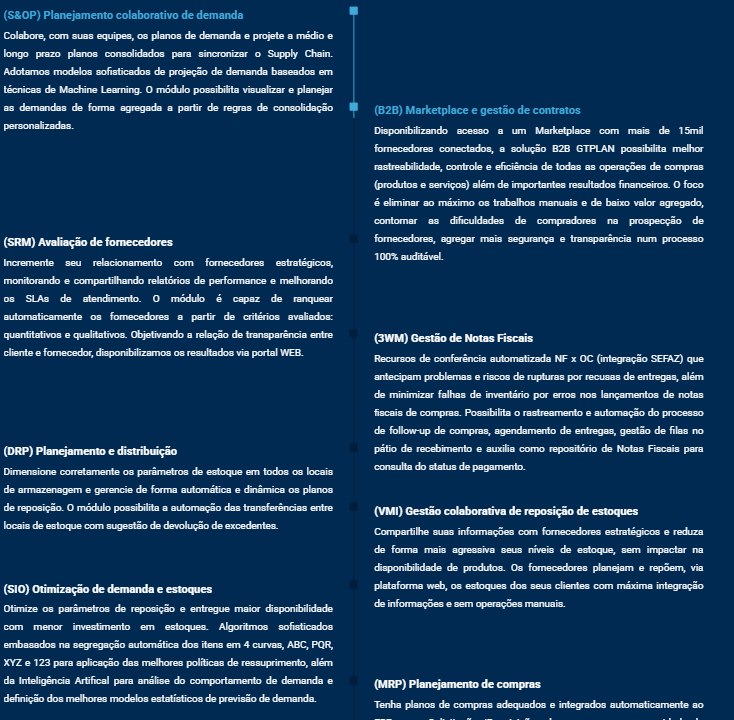
\includegraphics[width=0.6\linewidth]{Imagens/Benchmark/GTPlan.png}
    \caption{Soluções oferecidas pelo sistema GTPlan}
    \label{fig:gtplan}
\end{figure}

\subsubsection{Bionexo}

\begin{itemize}
    \item \textbf{Link:} https://bionexo.com/
    \item \textbf{Público-alvo:} Gestão de compras, cotações e estoque hospitalar
    \item \textbf{Funcionalidades principais:}
          \begin{itemize}
              \item Gestão de compras e cotações
              \item BioNFe (integração fiscal)
              \item Gestão de OPMEs
              \item BI e analytics (Bioanalytics)
              \item Planejamento (Plannexo)
          \end{itemize}
\end{itemize}

\begin{figure}[H]
    \centering
    \includegraphics[width=0.6\linewidth]{Imagens/Benchmark/Bionexo.png}
    \caption{Soluções oferecidas pela Bionexo}
    \label{fig:bionexo}
\end{figure}

\subsubsection{Slimstock}

\begin{itemize}
    \item \textbf{Link:} https://www.slimstock.com/pt/solucoes/software-previsao-demanda/
    \item \textbf{Público-alvo:} Empresas de varejo, distribuição e supply chain que necessitam de previsão de demanda
    \item \textbf{Funcionalidades principais:}
          \begin{itemize}
              \item Previsão de demanda com base em dados históricos, sazonalidade e tendências de mercado
              \item Demand sensing com inteligência artificial para previsões de curto prazo
              \item Planejamento de demanda colaborativo
              \item Otimização de níveis de estoque
              \item Gestão de demanda por cliente e canal de venda
          \end{itemize}
\end{itemize}

\begin{figure}[H]
    \centering
    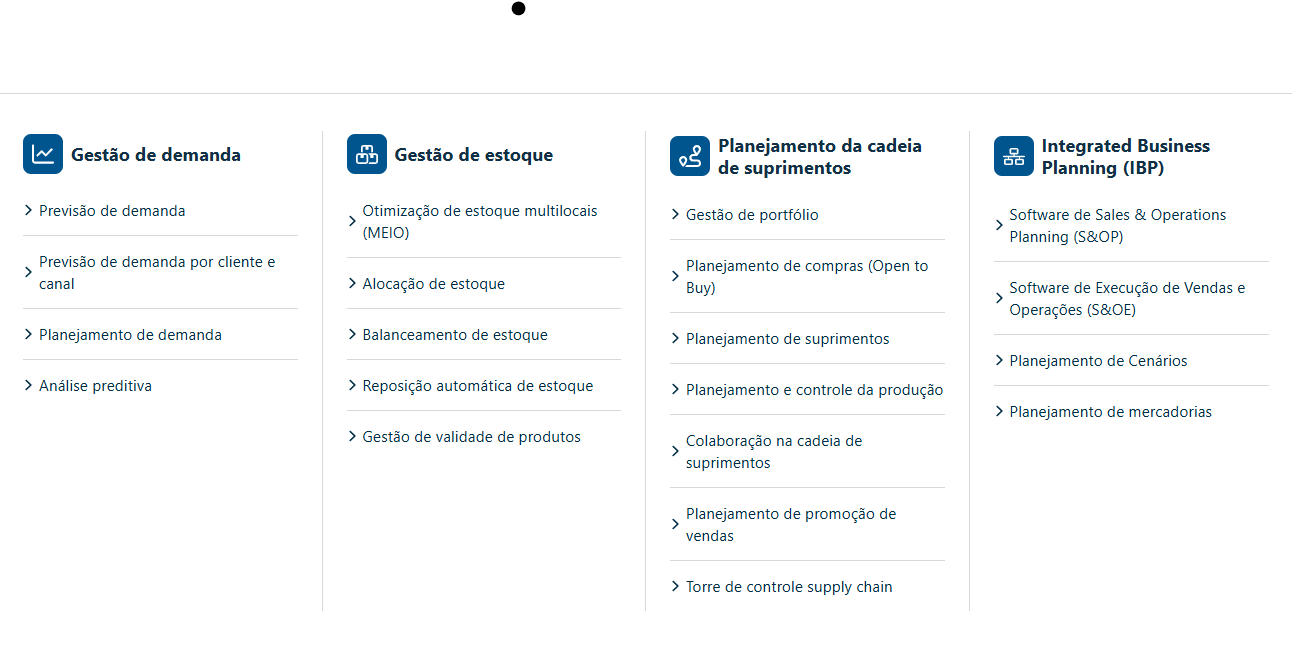
\includegraphics[width=0.6\linewidth]{Imagens/Benchmark/Slimstock.png}
    \caption{Soluções oferecidas pela Slimstock}
    \label{fig:slimstock}
\end{figure}

\subsubsection{o9 Solutions}

\begin{itemize}
    \item \textbf{Link:} https://o9solutions.com/solutions/demand-planning/ai-ml-forescasting
    \item \textbf{Público-alvo:} Grandes corporações com operações complexas de supply chain e planejamento de demanda
    \item \textbf{Funcionalidades principais:}
          \begin{itemize}
              \item Previsão de demanda com deep learning e modelos de Machine Learning automatizados
              \item Plataforma Digital Brain com tecnologia Graph Cube para relações complexas de dados
              \item Planejamento colaborativo de demanda em tempo real entre equipes
              \item Análise de Forecast Value Add (FVA) para medir impacto de cada etapa da previsão
              \item Segmentação multivariada com análise de ciclo de vida do produto
          \end{itemize}
\end{itemize}

\begin{figure}[H]
    \centering
    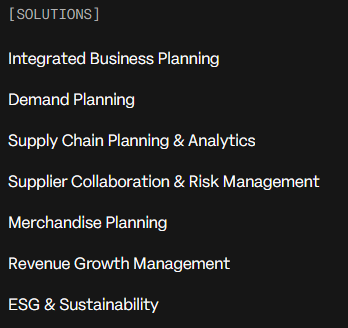
\includegraphics[width=0.6\linewidth]{Imagens/Benchmark/o9solutions.png}
    \caption{Soluções oferecidas pela o9 Solutions}
    \label{fig:o9solutions}
\end{figure}

\begin{longtable}{p{0.18\textwidth} p{0.38\textwidth} p{0.34\textwidth}}
    \toprule
    \textbf{Solução}                                                                                                                                                                                     & \textbf{Pontos Fortes} & \textbf{Limitações} \\
    \midrule
    \endfirsthead
    \toprule
    \textbf{Solução}                                                                                                                                                                                     & \textbf{Pontos Fortes} & \textbf{Limitações} \\
    \midrule
    \endhead
    GTPlan                                                                                                                                                                                               &
    Plataforma completa de gestão de suprimentos hospitalares; planejamento colaborativo de demanda; suporte a VMI e gestão de OPME; integração com BI e marketplace de fornecedores.                    &
    Solução enterprise de alto custo; não utiliza modelos de Machine Learning para previsão de demanda; requer infraestrutura e equipe dedicada.                                                                                                        \\
    \midrule
    Bionexo                                                                                                                                                                                              &
    Gestão integrada de compras e cotações hospitalares; integração fiscal (BioNFe); módulo de analytics (Bioanalytics); cobertura de OPMEs e planejamento (Plannexo).                                   &
    Foco principal no processo de compras, não em previsão de demanda; não utiliza Machine Learning; curva de adoção elevada.                                                                                                                           \\
    \midrule
    Slimstock                                                                                                                                                                                            &
    Previsão de demanda com IA e dados históricos; demand sensing de curto prazo; planejamento colaborativo; otimização de estoques.                                                                     &
    Voltada ao varejo e cadeia de mantimentos geral, sem especialização hospitalar; não cobre classificação ABC de insumos de saúde.                                                                                                                    \\
    \midrule
    o9 Solutions                                                                                                                                                                                         &
    Deep learning automatizado para previsão de demanda; plataforma Digital; planejamento colaborativo em tempo real; análise FVA.                                                                       &
    Plataforma enterprise de alta complexidade e custo elevado; voltada a grandes corporações; não é específica para o setor hospitalar.                                                                                                                \\
    \midrule
    Projeto Proposto                                                                                                                                                                                     &
    Foco exclusivo em previsão de consumo hospitalar com Machine Learning; classificação ABC dos itens; interface acessível para não técnicos; solução leve e de fácil adoção; exportação de relatórios. &
    Protótipo acadêmico sem módulos de compras ou gestão de fornecedores; dependente da qualidade dos dados históricos fornecidos.                                                                                                                      \\
    \bottomrule
\end{longtable}

\subsubsection{Diferencial do Projeto}

As soluções analisadas no benchmark revelam dois perfis distintos. GTPlan e Bionexo são plataformas voltadas especificamente ao setor hospitalar, com foco em gestão de compras e suprimentos, mas sem utilizar modelos de Machine Learning para previsão de demanda. Slimstock e o9 Solutions, por outro lado, aplicam IA e ML para previsão de demanda, porém são direcionadas ao varejo e grandes corporações, sem especialização no contexto hospitalar.

\noindent{O projeto proposto preenche essa lacuna ao oferecer uma solução especializada e de baixa complexidade operacional, com foco exclusivo na análise preditiva de consumo de insumos hospitalares. Enquanto as soluções existentes exigem grandes investimentos em implantação e infraestrutura, o sistema proposto é acessível, modular e voltado especificamente para apoiar a tomada de decisão de gestores hospitalares que necessitam de previsões de demanda confiáveis sem depender de plataformas complexas.}

\noindent{O nicho atendido são hospitais e instituições de saúde que já possuem dados históricos de consumo, mas não dispõem de ferramentas analíticas para transformá-los em previsões de demanda acionáveis, resultando em decisões de compra reativas e ineficientes.}

\subsection{Público-Alvo}

O sistema será utilizado por gestores hospitalares das áreas de compras, suprimentos e administração. A partir das previsões geradas pelos modelos de análise de dados, os gestores poderão avaliar tendências de consumo e utilizar essas informações para apoiar decisões relacionadas ao planejamento de compras e reposição de estoque.

\subsection{Objetivos do Projeto}

\subsubsection{Objetivo Geral}

O objetivo deste projeto é coletar e analisar dados históricos de consumo hospitalar, realizando o tratamento e a identificação de padrões de consumo. A partir desses padrões, serão aplicados modelos de aprendizado de máquina adequados para a realização de previsões de demanda. Por fim, os modelos serão avaliados por meio de métricas de desempenho, permitindo identificar quais abordagens apresentam melhores resultados para o problema proposto.

\subsubsection{Objetivos Específicos}

\begin{itemize}
    \item Automatizar o processo de análise de consumo de insumos hospitalares a partir de dados históricos;
    \item Permitir a análise exploratória dos dados de consumo, identificando padrões e tendências;
    \item Desenvolver modelos preditivos para estimar o consumo futuro de materiais e medicamentos;
    \item Disponibilizar um painel interativo para visualização de indicadores e previsões;
    \item Apoiar a tomada de decisão dos gestores por meio de informações analíticas e previsões de demanda.
\end{itemize}

\subsection{Métricas de Sucesso (KPIs)}

O sucesso do projeto será avaliado por meio de indicadores divididos em
duas categorias: desempenho dos modelos preditivos e desempenho do sistema.

\vspace{0.3cm}
\noindent\textbf{Desempenho dos Modelos Preditivos}

\begin{center}
    \begin{tabular}{p{0.18\textwidth} p{0.42\textwidth} p{0.28\textwidth}}
        \toprule
        \textbf{Métrica}                                            & \textbf{Descrição}                                              & \textbf{Meta} \\
        \midrule
        MAPE                                                        & Erro percentual médio absoluto entre o valor previsto e o real.
        Indica o quão próximas estão as previsões do consumo real.  &
        Inferior a 20\%                                                                                                                               \\
        \midrule
        MAE                                                         & Erro absoluto médio em unidades de consumo.
        Mede o desvio médio das previsões sem penalizar outliers.   &
        Minimizar em relação ao modelo baseline                                                                                                       \\
        \midrule
        RMSE                                                        & Raiz do erro quadrático médio.
        Penaliza erros maiores, indicando a estabilidade do modelo. &
        Minimizar em relação ao modelo baseline                                                                                                       \\
        \bottomrule
    \end{tabular}
\end{center}

\vspace{0.3cm}
\noindent\textbf{Desempenho do Sistema}

\begin{center}
    \begin{tabular}{p{0.18\textwidth} p{0.42\textwidth} p{0.28\textwidth}}
        \toprule
        \textbf{Indicador}                  & \textbf{Descrição}                           & \textbf{Meta} \\
        \midrule
        Tempo de resposta                   & Tempo de carregamento das páginas principais
        em condições normais de uso.        & Até 3 segundos                                               \\
        \midrule
        Tempo de predição                   & Tempo para geração de previsões para um
        conjunto padrão de até 1.000 itens. & Até 60 segundos                                              \\
        \midrule
        Cobertura de itens                  & Percentual de itens com histórico suficiente
        para geração de previsão.           & Mínimo de 80\% dos itens importados                          \\
        \bottomrule
    \end{tabular}
\end{center}

\section{Engenharia de Requisitos}

\subsection{Personas}

\noindent{Persona 1º - José:}
\begin{itemize}
    \item contexto: José é um diretor hospitalar responsável pela gestão de recursos e tomada de decisões estratégicas.
    \item objetivos: José deseja obter a visualização da previsão de consumo do seu hospital.
    \item principais dificuldades:
          \begin{itemize}
              \item Falta de previsibilidade no consumo de insumos hospitalares;
              \item Dificuldade na tomada de decisão baseada em dados históricos;
              \item Risco de falta ou excesso de materiais no hospital.
          \end{itemize}
\end{itemize}

\noindent{Persona 2º - Mônica:}
\begin{itemize}
    \item contexto: Mônica é supervisora do setor de estoque da farmácia hospitalar.
    \item objetivos: Mônica deseja visualizar qual será a previsão de consumo para o estoque da farmácia, conseguindo se organizar para alta demanda de um medicamento específico.
    \item principais dificuldades:
          \begin{itemize}
              \item Dificuldade em prever aumento repentino na demanda;
              \item Controle manual do estoque;
              \item Risco de vencimento de medicamentos devido à falta de planejamento.
          \end{itemize}
\end{itemize}

\noindent{Persona 3º - João:}
\begin{itemize}
    \item contexto: João é supervisor do setor de compras do hospital.
    \item objetivos: João deseja verificar qual será a previsão de consumo para se organizar nas solicitações de compras de determinados itens.
    \item principais dificuldades:
          \begin{itemize}
              \item Falta de dados confiáveis para planejamento de compras;
              \item Compras emergenciais com custo elevado;
              \item Dificuldade em alinhar demanda com fornecedores.
          \end{itemize}
\end{itemize}

\noindent{Persona 4º - Carlos:}
\begin{itemize}
    \item \textbf{Contexto:} Carlos é o responsável técnico pela plataforma,
          atuando como Super Admin do sistema. É o único com acesso ao painel de
          gestão de empresas e aprovação de novos hospitais.
    \item \textbf{Objetivos:}
          \begin{itemize}
              \item Cadastrar e gerenciar as empresas (hospitais) que utilizam
                    a plataforma;
              \item Aprovar ou rejeitar solicitações de acesso enviadas pelo
                    formulário de interesse;
              \item Garantir o correto isolamento dos dados entre as empresas
                    cadastradas.
          \end{itemize}
    \item \textbf{Principais dificuldades:}
          \begin{itemize}
              \item Necessidade de validar se a solicitação de acesso é legítima
                    antes de aprovar;
              \item Garantir que cada empresa tenha acesso apenas aos seus
                    próprios dados;
              \item Manter o controle sobre quais empresas estão ativas ou
                    inativas na plataforma.
          \end{itemize}
\end{itemize}

\subsection{Casos de Uso Principais}
Esta seção apresenta os principais casos de uso do sistema, organizados
por perfil de acesso. O primeiro diagrama ilustra as interações do perfil
Usuário, responsável pela consulta de previsões e visualização do dashboard.
O segundo diagrama apresenta as interações do perfil Administrador, que
possui acesso às funcionalidades de gestão e importação de dados.

\begin{figure}[H]
    \centering
    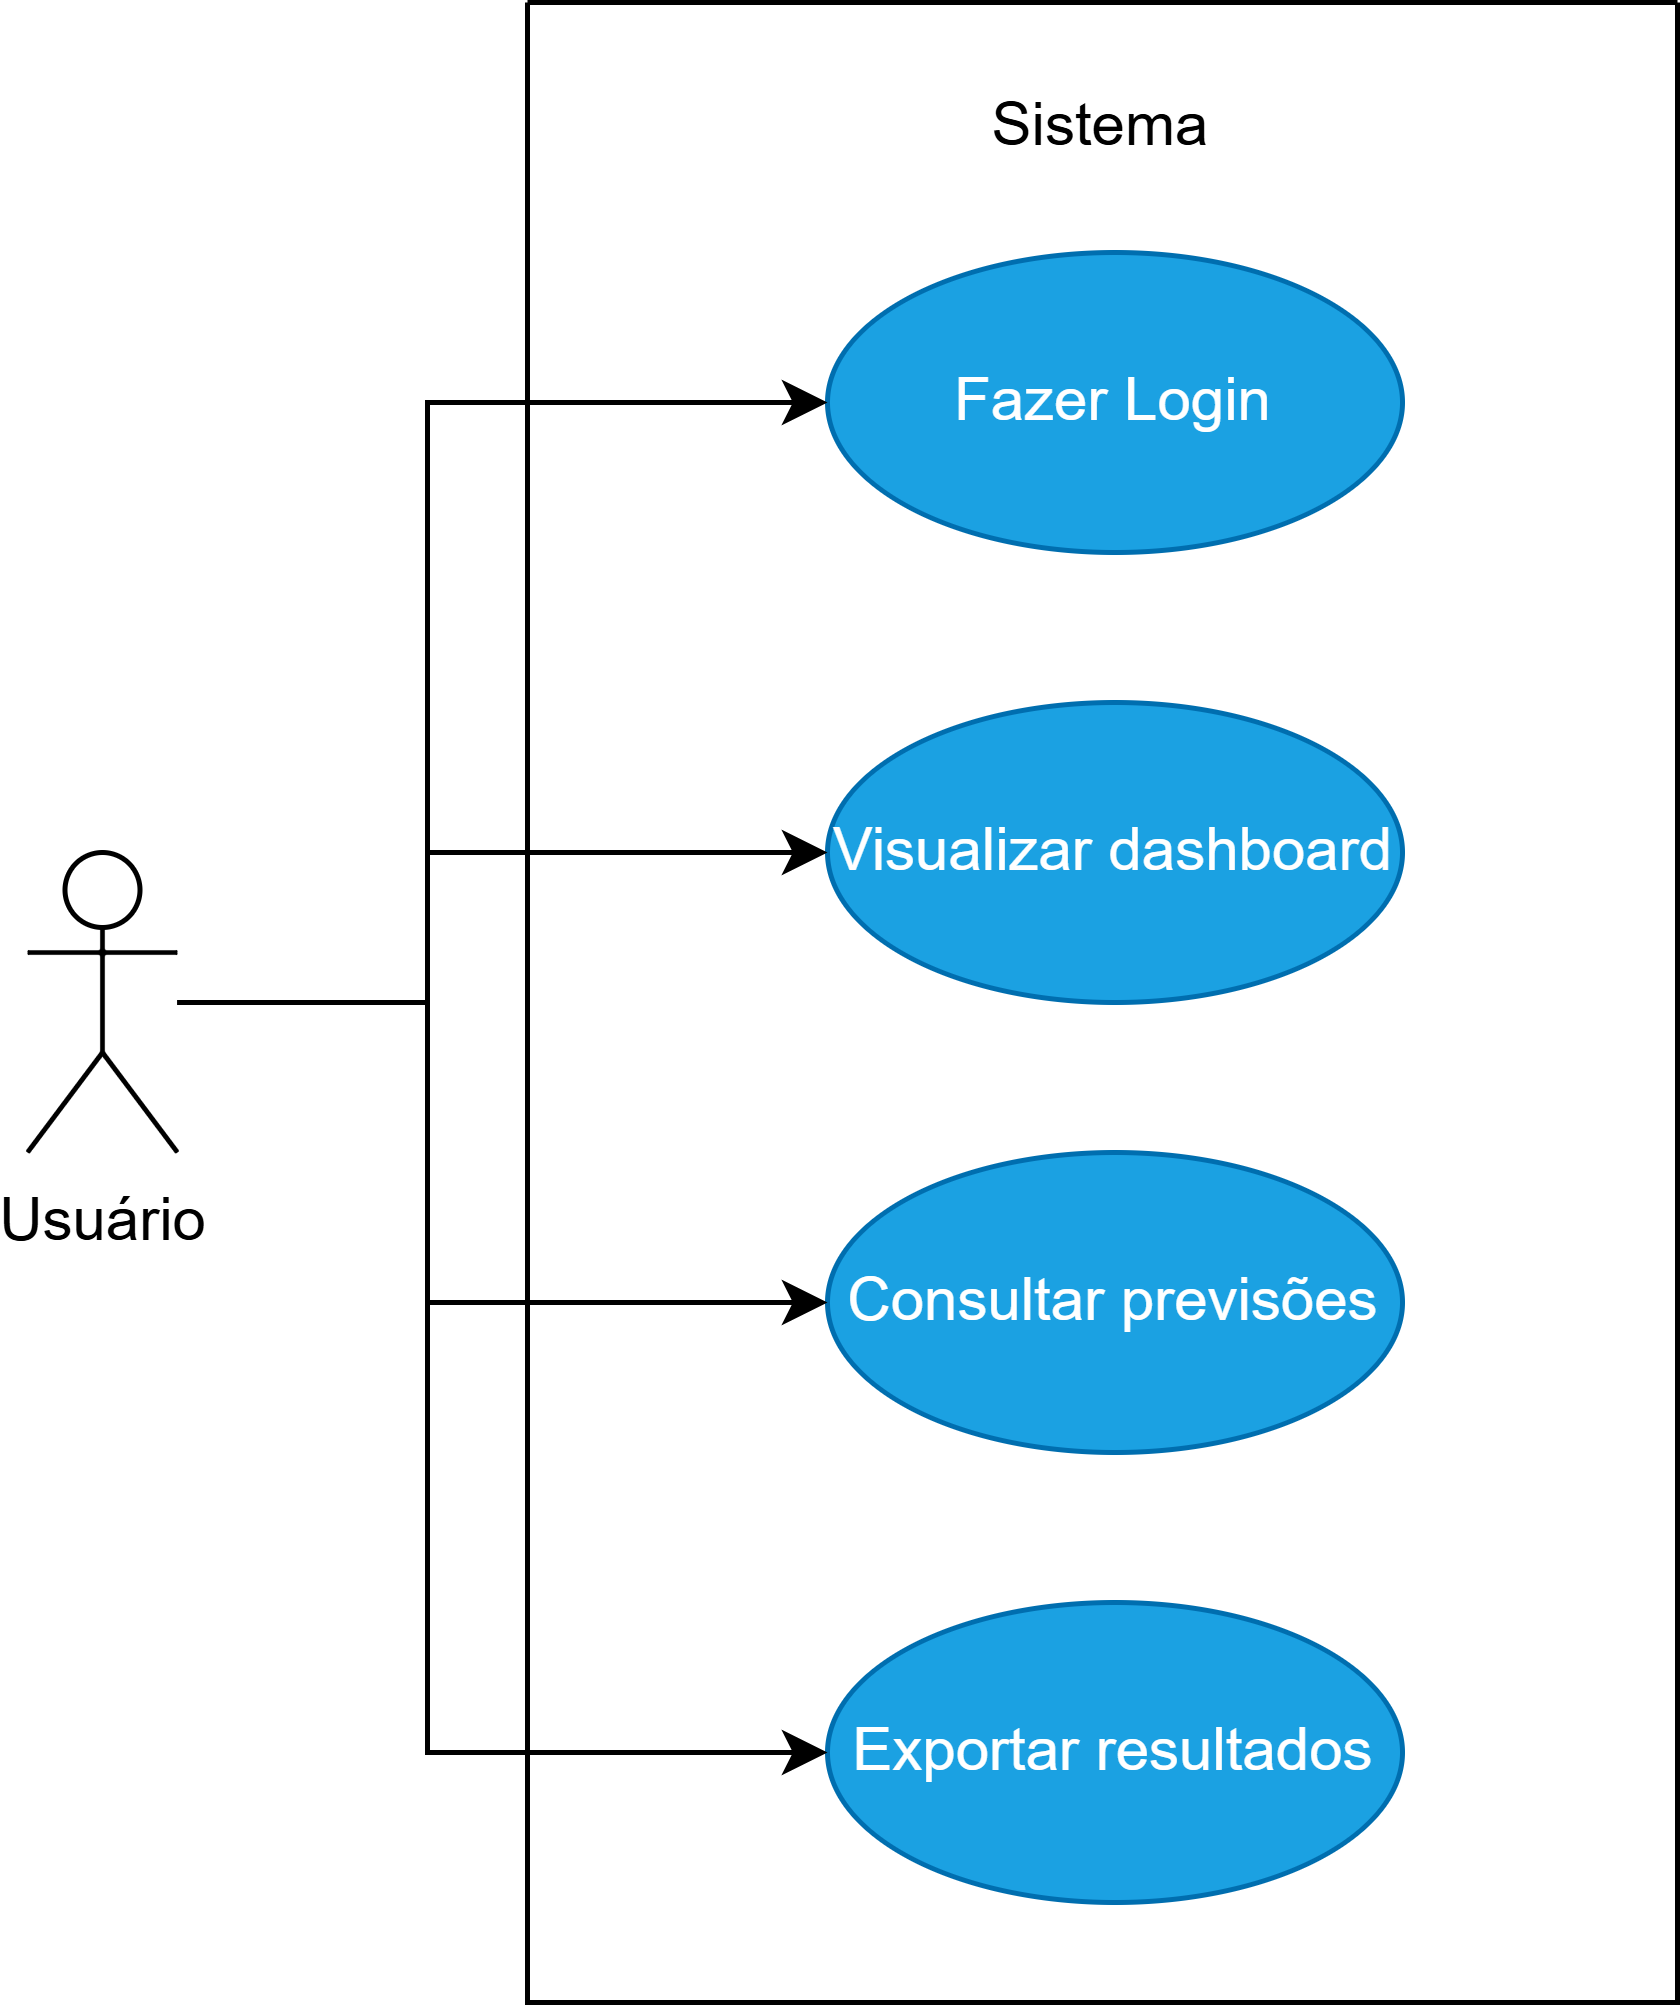
\includegraphics[width=0.8\textwidth]{Imagens/diagramas/Usuario_hospitalar_CDU.png}
    \caption{Diagrama de casos de uso do perfil Usuário, contemplando as funcionalidades de Login, Dashboard, Painel de Previsões e Painel de Relatório.}
\end{figure}

\begin{figure}[H]
    \centering
    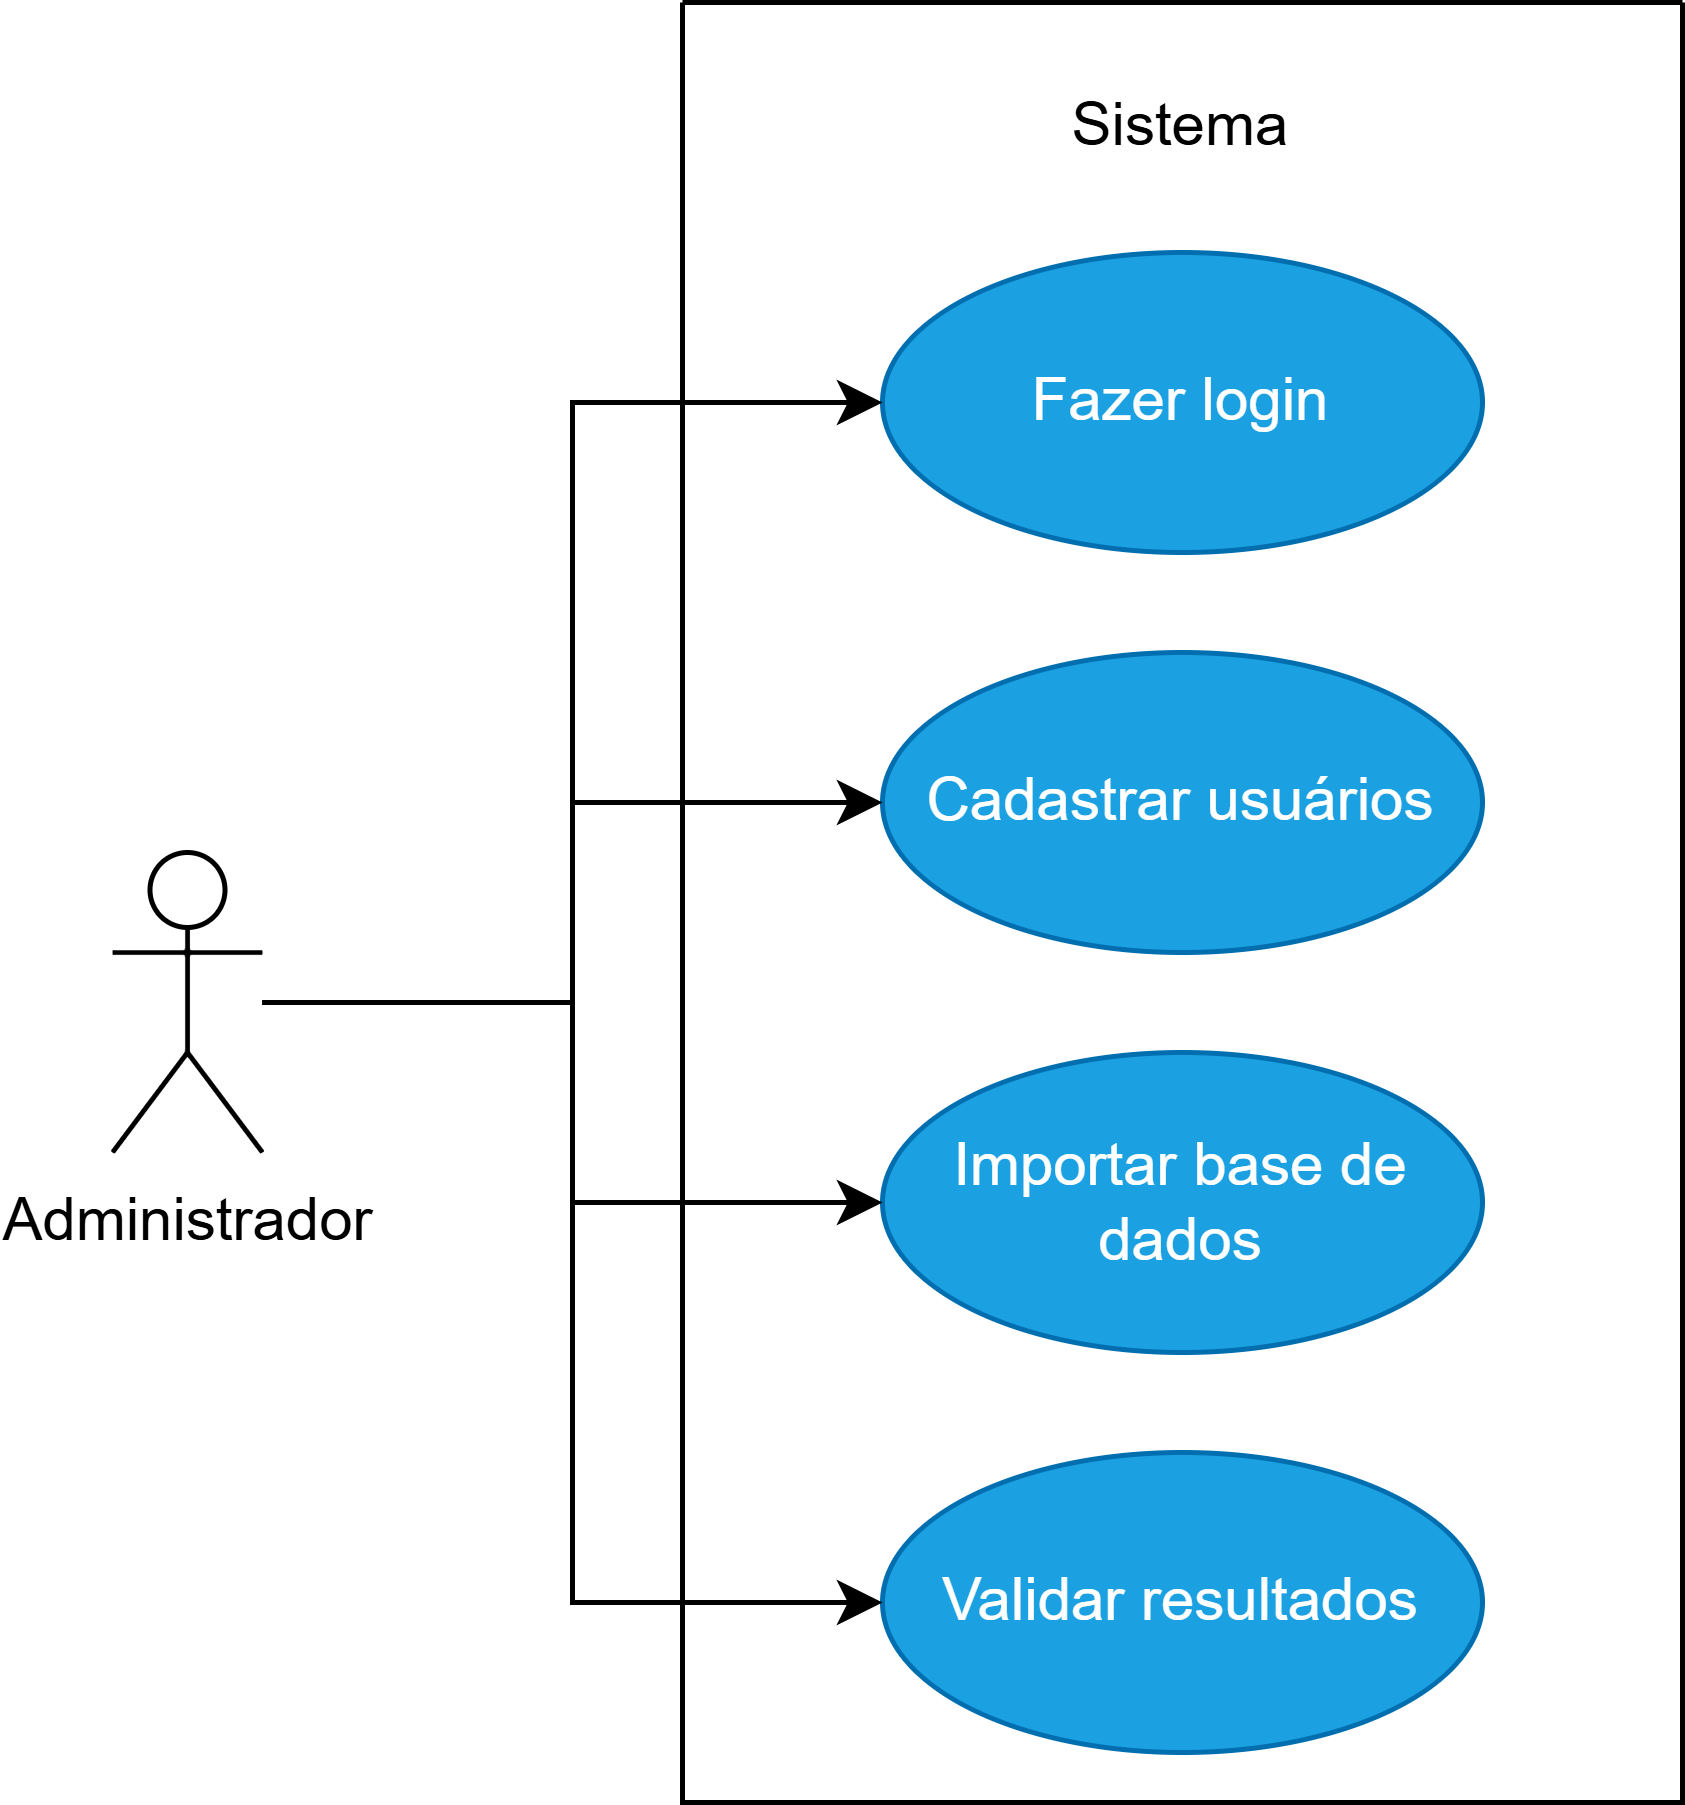
\includegraphics[width=0.8\textwidth]{Imagens/diagramas/Administrador_login_importar_dados_CDU.png}
    \caption{Diagrama de casos de uso do perfil Administrador, contemplando acesso completo ao sistema incluindo gestão de usuários e importação de dados.}
\end{figure}

\subsection{Requisitos Funcionais (RF)}

\begin{longtable}{p{0.18\textwidth} p{0.78\textwidth}}
    \toprule
    \textbf{Código} & \textbf{Descrição} \\
    \midrule
    \endfirsthead

    \toprule
    \textbf{Código} & \textbf{Descrição} \\
    \midrule
    \endhead

    \bottomrule
    \endfoot

    \rf{RF01}{O sistema deve permitir o cadastro e autenticação de usuários com perfis de acesso distintos, administrados e usuário.}
    \rf{RF02}{O sistema deve permitir a importação de bases históricas de
        consumo hospitalar nas seguintes modalidades:
        \begin{enumerate}[label=\alph*)]
            \item upload manual de arquivo nos formatos CSV ou Excel;
            \item integração via API REST com o sistema hospitalar legado (ERP),
                  com periodicidade de carga configurável pelo Administrador.
        \end{enumerate}
    }
    \rf{RF03}{O sistema deve permitir a visualização dos dados importados em tabelas e gráficos.}
    \rf{RF04}{O sistema deve realizar validações básicas nos dados importados, como identificação de valores nulos e inconsistências.
        \begin{enumerate}[label=\alph*)]
            \item extração dos dados da fonte integrada;
            \item padronização de nomes de campos e tipos de dados;
            \item tratamento de valores nulos;
            \item remoção de duplicidades;
            \item detecção de inconsistências de formato, datas e quantidades;
            \item agregação temporal dos dados para análise e previsão;
            \item armazenamento dos dados tratados para uso analítico e preditivo.
        \end{enumerate}
    }
    \rf{RF05}{O sistema deve permitir a classificação dos itens conforme padrões de consumo definidos no projeto, como as classificações ABC e a classificação combinada ABC.}
    \rf{RF06}{O sistema deve disponibilizar um pipeline de treinamento de modelos preditivos, contemplando no mínimo:
        \begin{enumerate}[label=\alph*)]
            \item ingestão dos dados tratados;
            \item seleção e preparação das variáveis;
            \item engenharia de atributos;
            \item separação entre dados de treino, validação e teste;
            \item treinamento dos modelos de Machine Learning e séries temporais;
            \item avaliação com métricas definidas;
            \item registro dos resultados de treinamento.
        \end{enumerate}
    }
    \rf{RF07}{O sistema deve apresentar o desempenho dos modelos testados com base em métricas como RMSE, MAE e MAPE.}
    \rf{RF08}{O sistema deve gerar previsões de consumo futuro para matérias e medicamentos.}
    \rf{RF09}{O sistema deve apresentar um painel com gráficos, de forma a apoiar a tomada de decisão sobre estoque hospitalar.}
    \rf{RF10}{O sistema deve permitir a exportação dos resultados das previsões e métricas em formato PDF.}
    \rf{RF11}{O sistema deve permitir o retreinamento dos modelos a partir de novos dados históricos, de forma manual ou programada, mantendo registro de versões de modelo e resultados obtidos.}
    \rf{RF12}{O sistema deve exibir uma mensagem informativa no Dashboard quando não houver dados importados, orientando o usuário a realizar a primeira importação.}
    \rf{RF13}{O sistema deve permitir que o Super Admin cadastre, edite e desative empresas (hospitais).}
    \rf{RF14}{O sistema deve exibir na tela de login um botão de interesse, permitindo que um hospital informe e-mail, nome do responsável e nome do hospital.}
    \rf{RF15}{O sistema deve permitir que o Super Admin visualize, aprove ou rejeite solicitações de acesso recebidas.}
    \rf{RF16}{O sistema deve garantir isolamento total dos dados entre empresas, assegurando que usuários de uma empresa não acessem dados de outra.}
\end{longtable}

\subsection{Requisitos Não Funcionais (RNF)}

\begin{longtable}{p{0.18\textwidth} p{0.72\textwidth}}
    \toprule
    \textbf{Código} & \textbf{Descrição} \\
    \midrule
    \endfirsthead
    \toprule
    \textbf{Código} & \textbf{Descrição} \\
    \midrule
    \endhead
    \rnf{RNF01}	{O sistema deve carregar as páginas principais em até 3 segundos em condições normais de uso.}
    \rnf{RNF02}	{O sistema deve gerar previsões para um conjunto padrão de até 1.000 itens em no máximo 60 segundos, considerando modelos já treinados (o treinamento e o retreinamento dos modelos seguem o RF11 e não estão sujeitos a este limite de tempo).}
    \rnf{RNF03}	{A interface do sistema deve ser intuitiva e permitir que usuários não técnicos compreendam os resultados apresentados.}
    \rnf{RNF04}	{O sistema deve exigir autenticação para acesso às funcionalidades restritas.}
    \rnf{RNF05}	{O sistema deve armazenar e processar apenas os dados necessários à finalidade proposta, em conformidade com a LGPD, garantindo minimização e proteção dos dados utilizados.}
    \rnf{RNF06}	{O sistema deve estar disponível para acesso durante o período de uso acadêmico e testes do projeto.}
    \rnf{RNF07}	{A arquitetura do sistema deve permitir integração com novas fontes de dados por meio de APIs e conectores, sem necessidade de reestruturação completa da aplicação.}
    \rnf{RNF08}	{O código-fonte deve ser estruturado de forma modular, facilitando manutenção e evolução futura.}
    \rnf{RNF09}	{O sistema deve registrar logs de execução, erros de processamento e falhas de integração, permitindo rastreabilidade e auditoria técnica.}
    \rnf{RNF10}	{O sistema web deve funcionar nos principais navegadores atuais.}
    \rnf{RNF11}	{O sistema deve adotar comunicação segura entre cliente e servidor por meio de HTTPS.}
    \bottomrule
\end{longtable}

\subsection{Regras de Negócio}

\begin{longtable}{p{0.10\textwidth} p{0.20\textwidth} p{0.60\textwidth}}
    \toprule
    \textbf{Código} & \textbf{Categoria}  & \textbf{Descrição}                                                                                                                                                                                                                                                               \\
    \midrule
    \endfirsthead
    \toprule
    \textbf{Código} & \textbf{Categoria}  & \textbf{Descrição}                                                                                                                                                                                                                                                               \\
    \midrule
    \endhead

    RN01            & Controle de Acesso  & O sistema possui três perfis de acesso. O Super Admin gerencia empresas e aprova solicitações de acesso. O Administrador cadastra, edita e inativa usuários dentro da sua própria
    empresa. O Usuário acessa apenas as funcionalidades de consulta.                                                                                                                                                                                                                                                         \\\midrule

    RN02            & Controle de Acesso  & Apenas usuários com perfil Administrador podem realizar importações de dados, ficando restritos exclusivamente aos dados da empresa à qual pertencem.                                                                                                                            \\\midrule

    RN03            & Validação de Dados  & Os arquivos importados devem conter obrigatoriamente as colunas: código do item, descrição do item, data, quantidade de consumo e local de estoque. Caso alguma dessas colunas não seja identificada, a importação é rejeitada e o usuário é notificado com a descrição do erro. \\\midrule

    RN04            & Exportação          & A exportação de relatórios está disponível para todos os perfis de usuário, nos formatos PDF e Excel (.xlsx).                                                                                                                                                                    \\\midrule

    RN05            & Classificação ABC   & A classificação ABC dos itens segue as faixas de mercado: Classe A — primeiros 70\% do valor acumulado de consumo; Classe B — próximos 20\%; Classe C — últimos 10\%.                                                                                                            \\\midrule

    RN06            & Modelo Preditivo    & O sistema somente gera previsões para itens que possuam histórico de consumo de no mínimo 3 meses de dados válidos após o tratamento.                                                                                                                                            \\\midrule

    RN07            & Dashboard           & O sistema deve exibir uma mensagem informativa no Dashboard quando não houver dados importados, orientando o usuário a realizar a primeira importação.                                                                                                                           \\\midrule

    RN08            & Isolamento de Dados & Cada empresa acessa exclusivamente seus próprios dados; nenhum usuário pode visualizar ou manipular dados de outra empresa                                                                                                                                                       \\\midrule

    RN09            & Gestão de Empresas  & Somente o Super Admin pode cadastrar, editar e desativar empresas no sistema.                                                                                                                                                                                                    \\\midrule

    RN10            & Aprovação de Acesso & Solicitações de interesse recebidas pelo formulário do login ficam com status "pendente" até aprovação ou rejeição explícita pelo Super Admin                                                                                                                                    \\\midrule

    RN11            & Conta Super Admin   & As credenciais do Super Admin são configuradas via variável de ambiente e gerenciadas fora do banco de dados de usuários comuns, não sendo possível criá-las ou alterá-las pela interface do sistema                                                                             \\

    \bottomrule
\end{longtable}

\subsection{Fora do Escopo}

O projeto apresenta algumas limitações que devem ser consideradas. A primeira refere-se à dependência da qualidade dos dados históricos, uma vez que inconsistências ou dados incompletos podem afetar o desempenho dos modelos de previsão.\\

\noindent{Outra limitação está relacionada à possível dificuldade de integração com sistemas hospitalares
    existentes uma vez que diferentes instituições utilizam sistemas de gestão distintos.}\\

\noindent{Além disso, o escopo do projeto poderá ser limitado a determinados tipos de insumos hospitalares, não abrangendo necessariamente todos os materiais utilizados em um hospital.}

% -------------------------------------------------
\section{Fluxos e Comportamento do Sistema}

\subsection{Fluxo Principal do Usuário}

O diagrama a seguir apresenta o fluxo principal do usuário no sistema.
\begin{figure}[H]
    \centering
    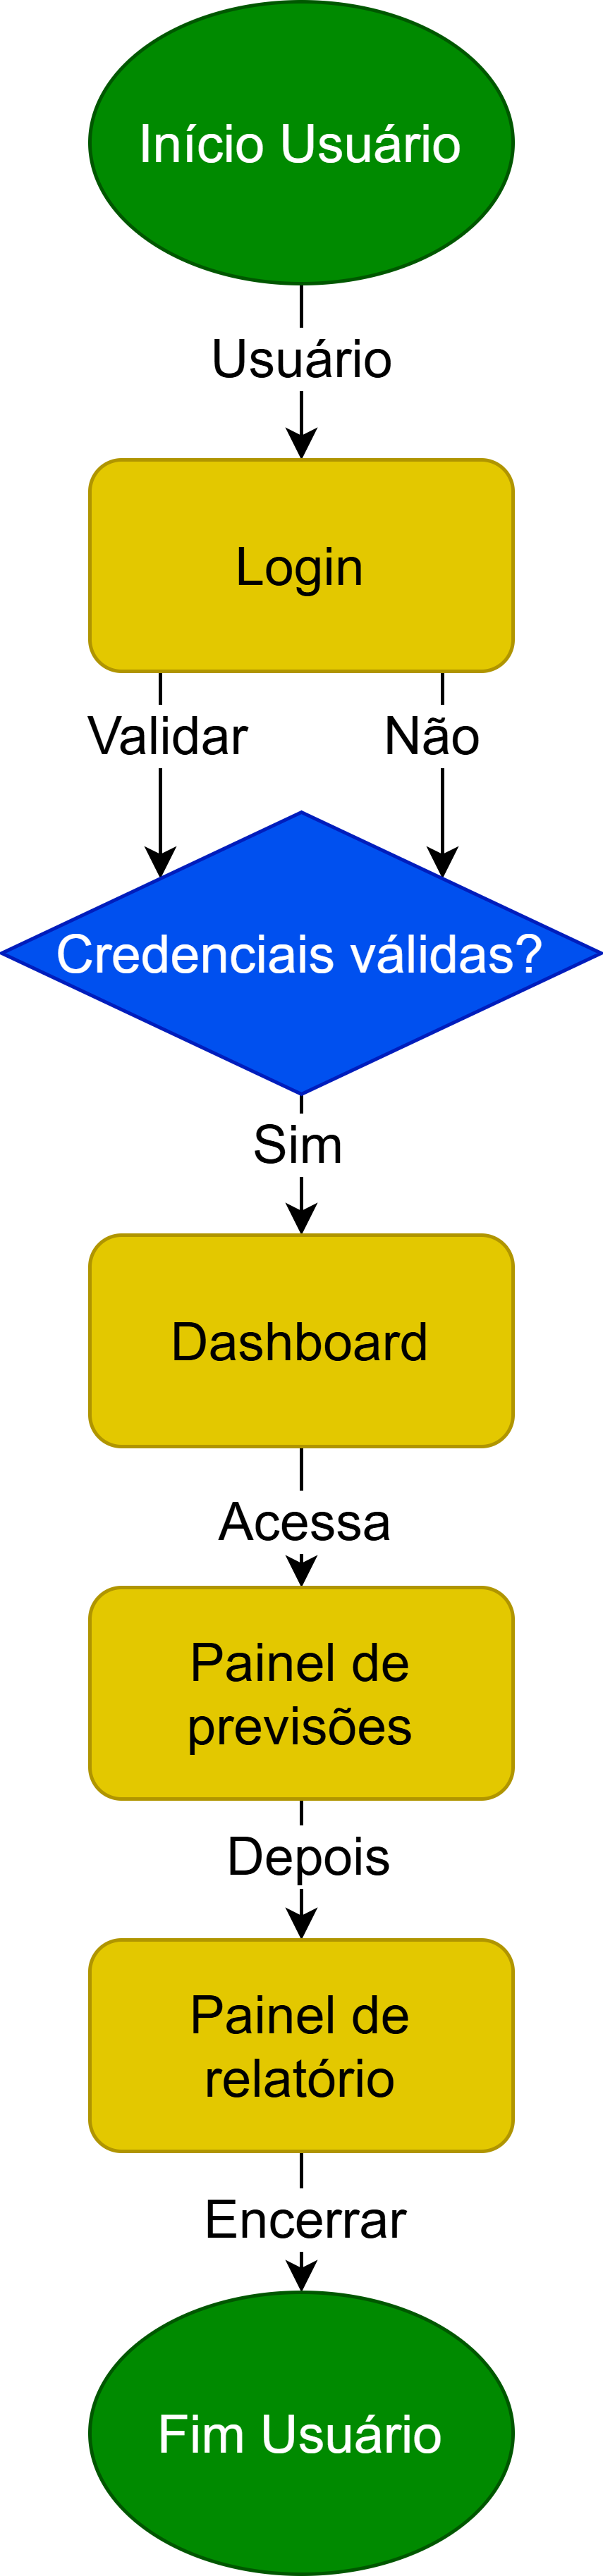
\includegraphics[width=0.2\textwidth]{Imagens/diagramas/Atividades_usuario.png}
    \caption{Diagrama de atividades do fluxo principal do usuário, desde a autenticação até a visualização do painel de relatórios.}
    \label{fig:fluxo-usuario}
\end{figure}

\subsection{Fluxo Principal do Administrador}

O diagrama a seguir apresenta o fluxo principal do administrador no sistema.
\begin{figure}[H]
    \centering
    \includegraphics[width=0.75\textwidth]{Imagens/diagramas/atividades_administrador.png}
    \caption{Diagrama de atividades do fluxo principal do administrador, desde a autenticação até a importação de dados no sistema.}
    \label{fig:fluxo-administrador}
\end{figure}

\subsection{Fluxos Alternativos}

\vspace{0.4cm}
\noindent\textbf{FA01 — Credenciais inválidas no Login} \\
\textbf{Condição:} O usuário informa e-mail ou senha incorretos. \\
\textbf{Resposta do sistema:} Exibe mensagem de erro informando credenciais
inválidas e permite nova tentativa. O acesso não é concedido.

\vspace{0.4cm}
\noindent\textbf{FA02 — Arquivo de importação inválido} \\
\textbf{Condição:} O arquivo CSV não contém as colunas obrigatórias ou
possui dados corrompidos. \\
\textbf{Resposta do sistema:} Rejeita a importação, exibe a descrição do
erro ao Administrador e mantém o histórico de dados anterior intacto.

\vspace{0.4cm}
\noindent\textbf{FA03 — Dados insuficientes para previsão} \\
\textbf{Condição:} Um ou mais itens possuem menos de 3 meses de histórico
de consumo válido. \\
\textbf{Resposta do sistema:} Gera previsões apenas para os itens com
histórico suficiente e exibe aviso indicando quais itens foram omitidos.

\vspace{0.4cm}
\noindent\textbf{FA04 — Sessão expirada} \\
\textbf{Condição:} O usuário permanece inativo por um período prolongado. \\
\textbf{Resposta do sistema:} Encerra a sessão automaticamente e redireciona
o usuário para a tela de Login.

\vspace{0.4cm}
\noindent\textbf{FA05 — Acesso não autorizado} \\
\textbf{Condição:} Um usuário com perfil Usuário tenta acessar uma
funcionalidade restrita ao Administrador. \\
\textbf{Resposta do sistema:} Bloqueia o acesso e exibe mensagem informando
que o usuário não possui permissão para acessar o recurso solicitado.

% -------------------------------------------------
\section{Mockups e Experiência do Usuário (UX)}

\subsection{Fluxo de Navegação}

O diagrama a seguir apresenta o fluxo de navegação entre as telas do sistema, evidenciando quais são acessíveis a todos os perfis de usuário e quais são restritas ao perfil Administrador.

\begin{figure}[H]
    \centering
    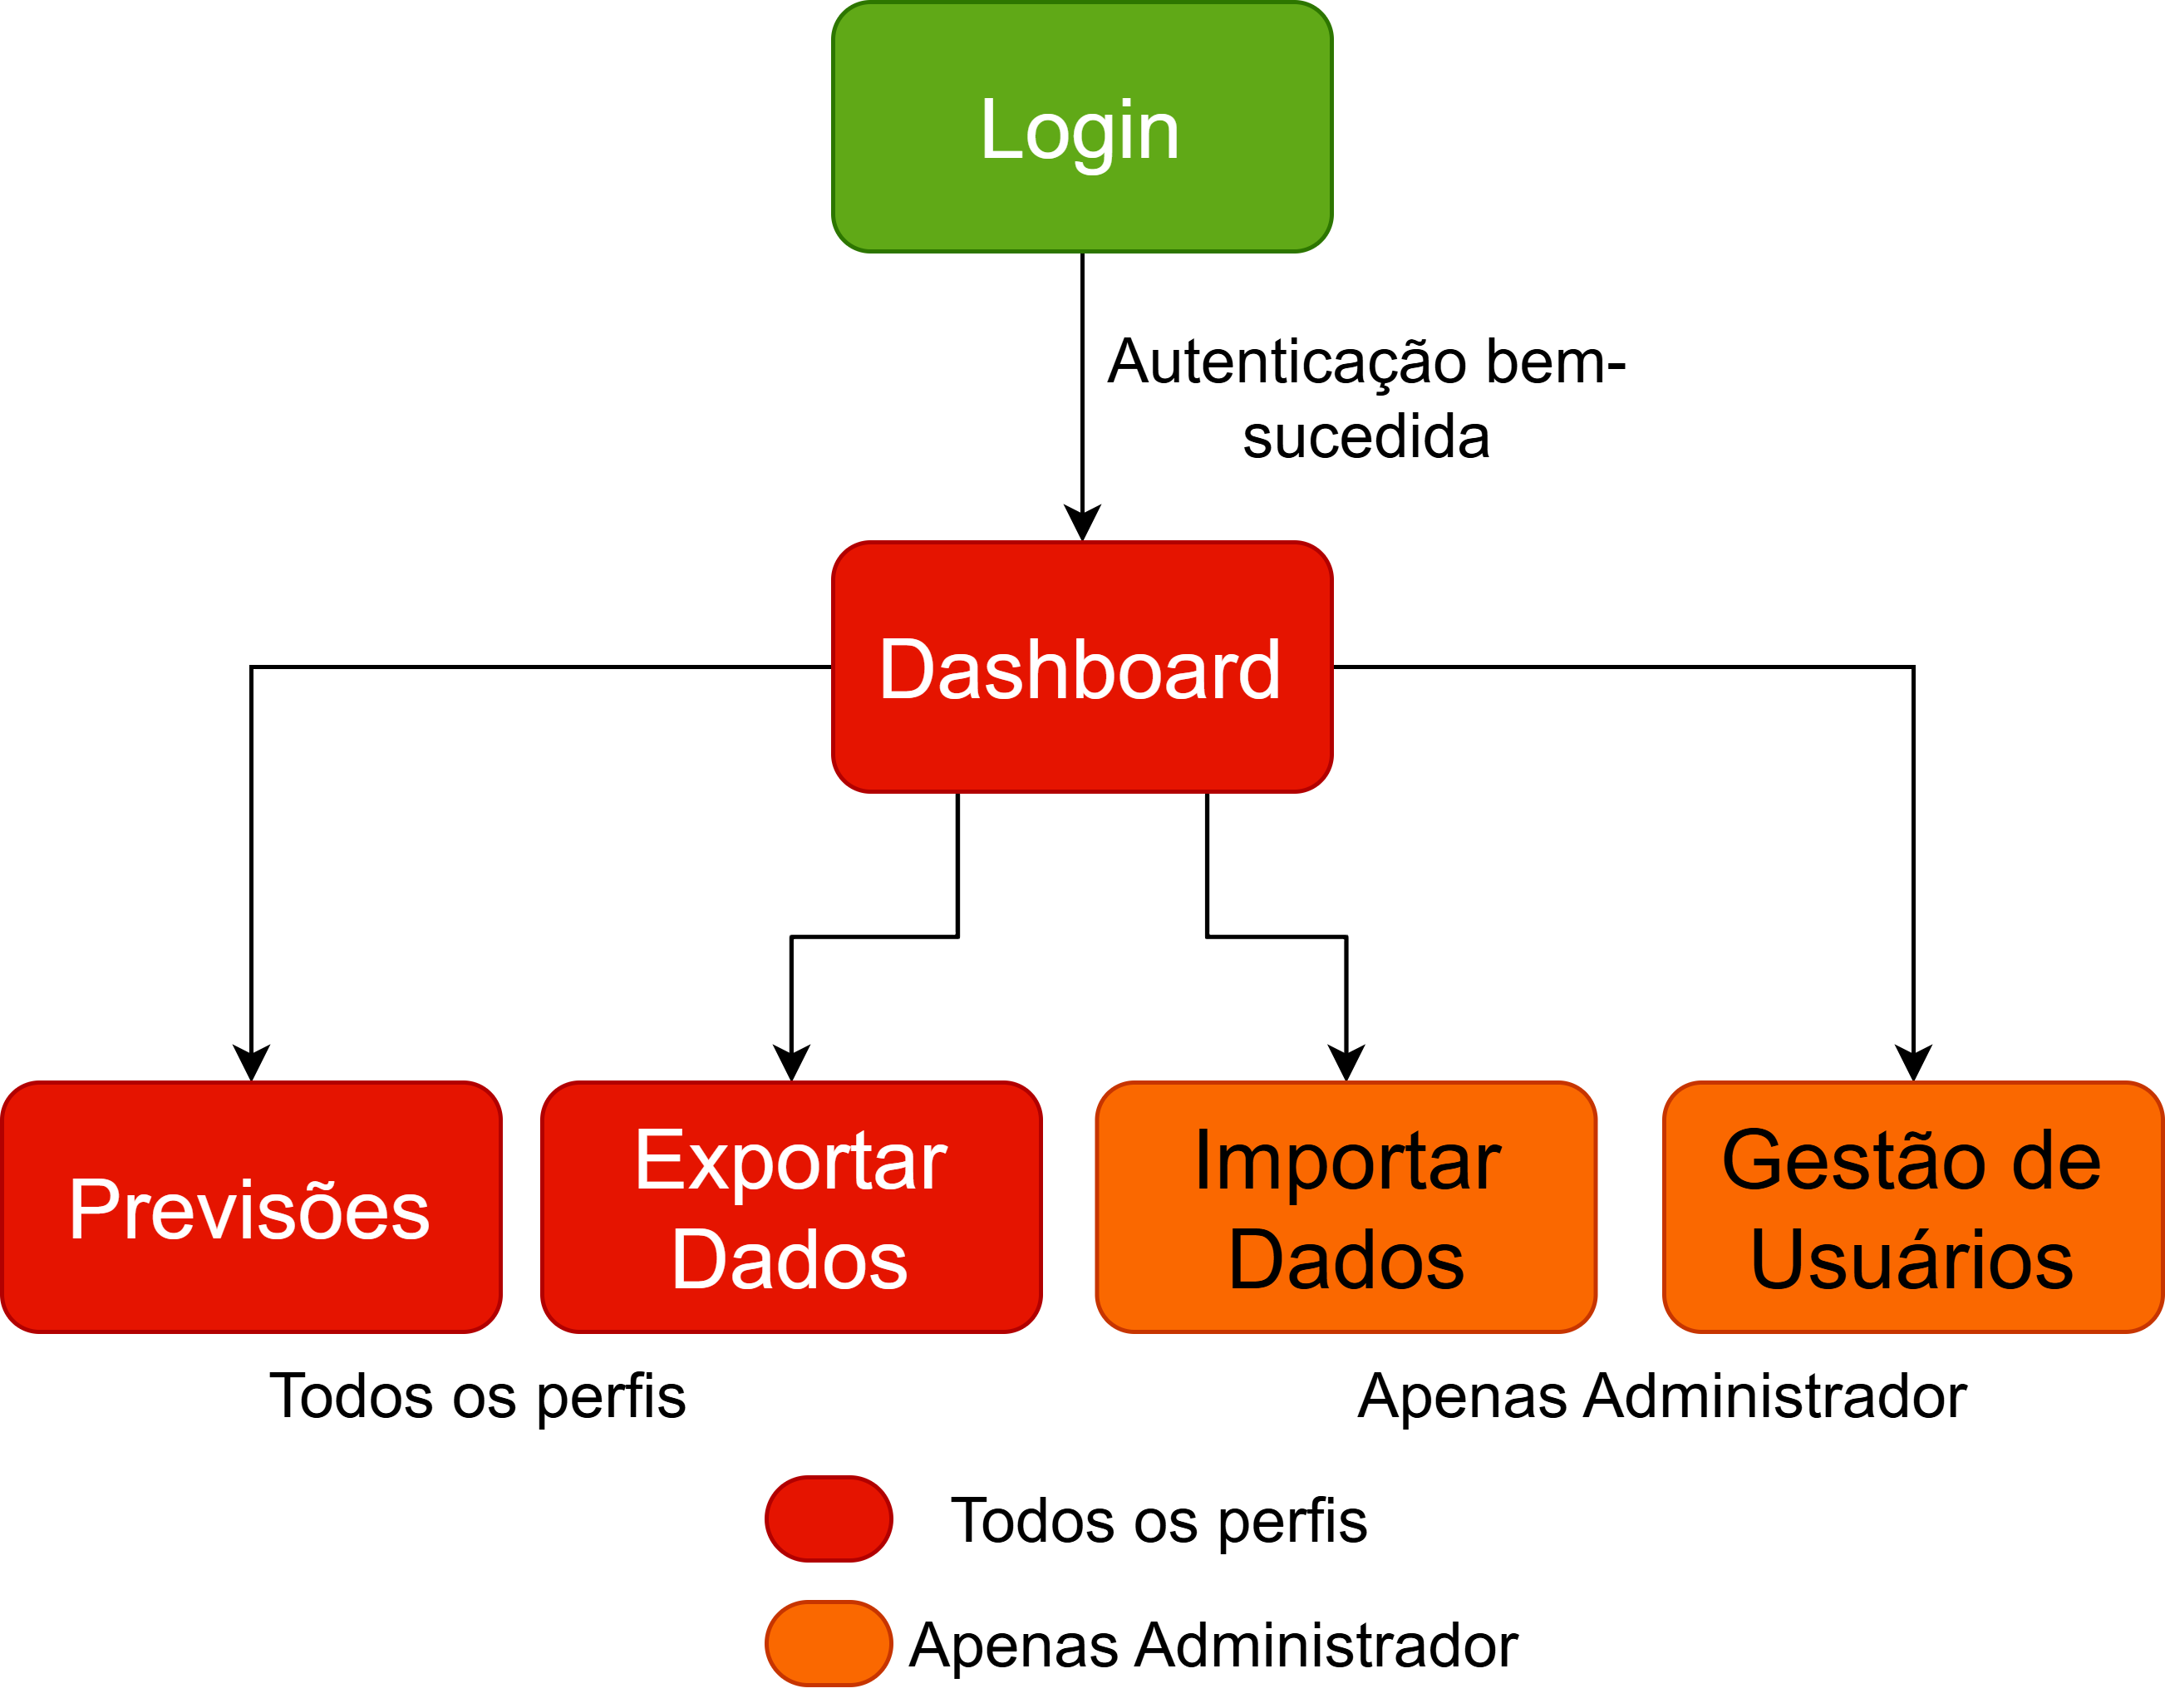
\includegraphics[width=0.95\textwidth]{Imagens/diagramas/TCC-fluxo_navegacao.png}
    \caption{Diagrama de navegação entre telas do sistema.}
    \label{fig:fluxo-navegacao}
\end{figure}

\noindent{A navegação parte sempre da tela de \textbf{Login}. A partir dela, novos hospitais podem acessar o formulário de \textbf{Solicitação de Acesso} sem necessidade de autenticação. Após autenticação bem-sucedida, o usuário é direcionado ao \textbf{Dashboard}, que funciona como hub central do sistema. A partir dele, todos os perfis podem acessar \textbf{Previsões} e \textbf{Exportar Relatório}. As telas de \textbf{Importar Dados} e \textbf{Gestão de Usuários} são acessíveis exclusivamente ao perfil Administrador. O perfil \textbf{Super Usuário} acessa exclusivamente a tela de \textbf{Gestão de Hospitais}, onde gerencia as instituições cadastradas e analisa as solicitações de acesso pendentes.}

\subsection{Wireframes ou Mockups das Telas}

O sistema é composto por 5 telas principais, descritas a seguir com suas respectivas funcionalidades e ações disponíveis ao usuário.

\paragraph{Dashboard}
Inicialmente exibida vazia, pois ainda não há dados importados. Após a realização da importação, o dashboard é carregado com as principais visões: KPIs, gráficos de consumo mensal, consumo por local de estoque e classificação ABC dos itens.

\textit{Ações principais:} visualizar KPIs, analisar gráficos de consumo e acompanhar a classificação ABC dos itens.

\begin{figure}[H]
    \centering
    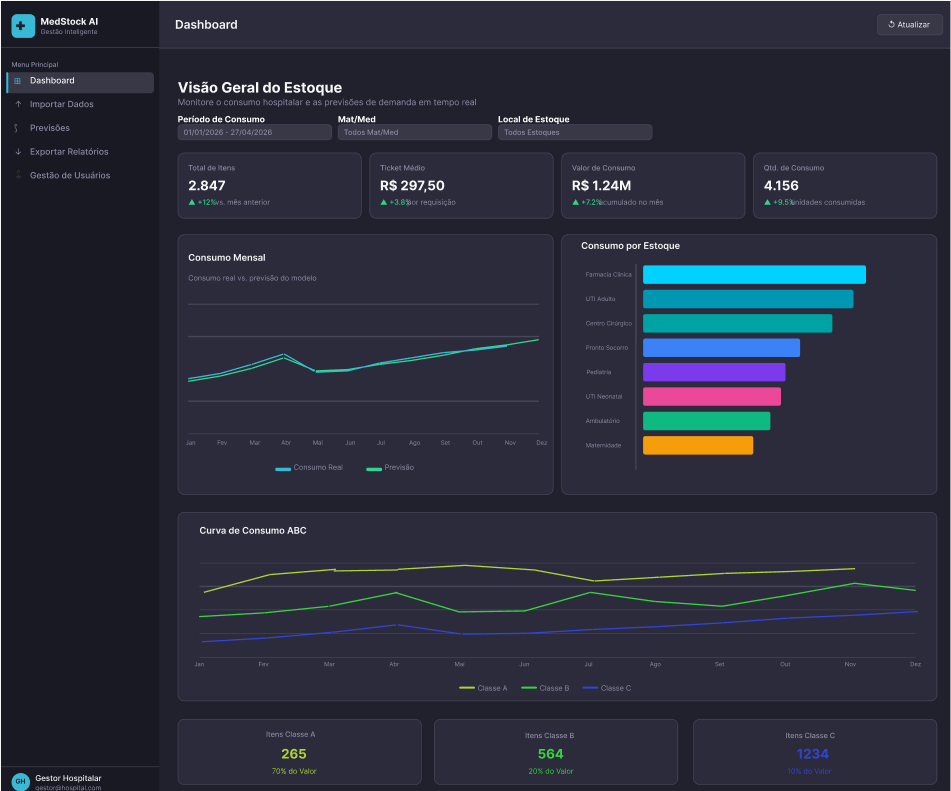
\includegraphics[width=0.8\textwidth]{Imagens/Mockups/Dasdboard.png}
    \caption{Tela de Dashboard.}
\end{figure}

\paragraph{Importar Dados}
Tela destinada à importação de dados para a plataforma, em formato CSV ou por meio da configuração de uma API com periodicidade de carga programável. O sistema realiza validações automáticas (valores nulos, duplicidades, formato de datas, tipos de dados, inconsistências e agregação temporal) e exibe um histórico das importações realizadas.

\textit{Ações principais:} importar arquivo CSV, configurar integração via API, agendar periodicidade de carga e consultar histórico de importações.

\begin{figure}[H]
    \centering
    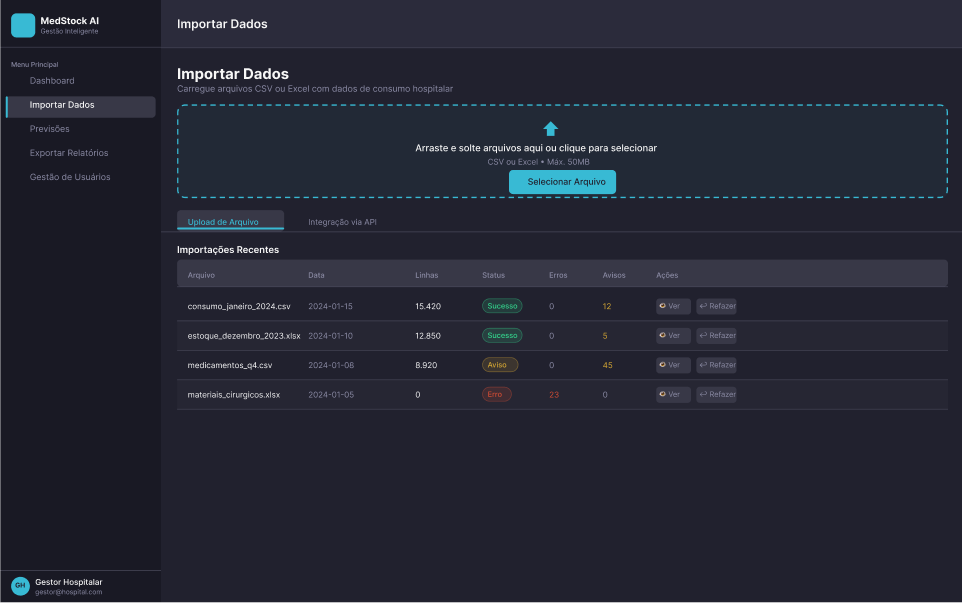
\includegraphics[width=0.8\textwidth]{Imagens/Mockups/Importar_Dados.png}
    \caption{Tela de Importar Dados.}
\end{figure}

\paragraph{Previsões}
Núcleo do sistema. Nesta tela é possível visualizar as previsões de consumo geradas pelos modelos preditivos, por meio de gráficos de tendência e uma tabela com os materiais e suas respectivas previsões.

\textit{Ações principais:} visualizar gráficos de previsão de consumo e consultar a tabela de materiais com suas previsões estimadas.

\begin{figure}[H]
    \centering
    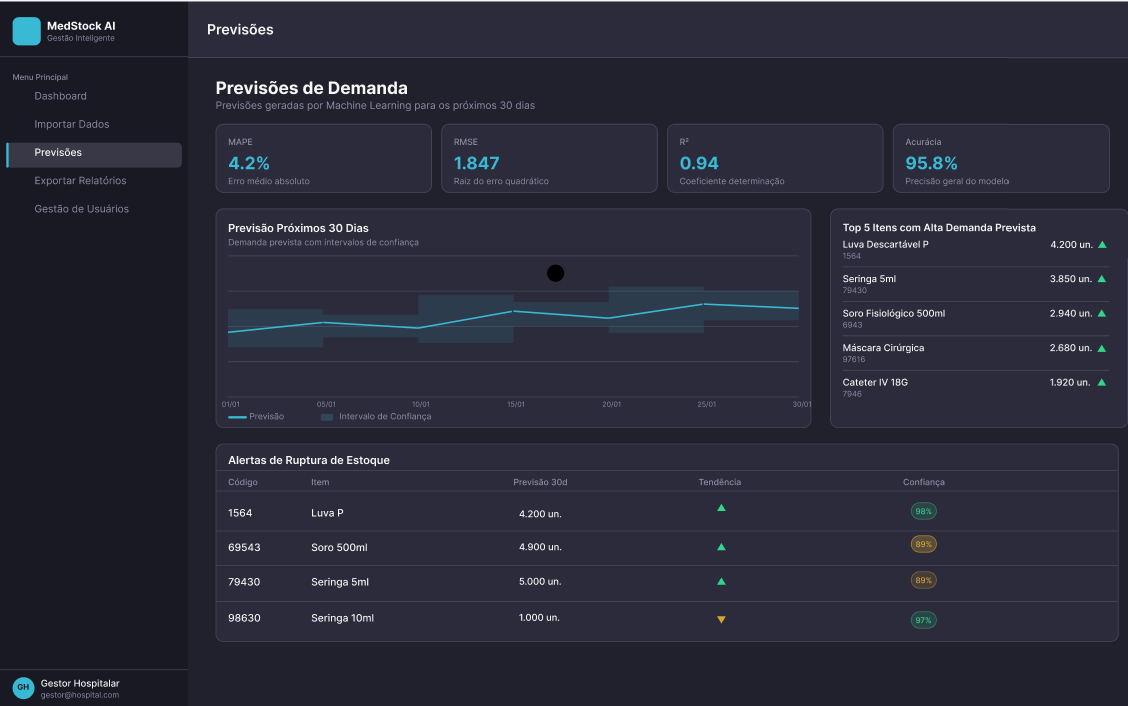
\includegraphics[width=0.8\textwidth]{Imagens/Mockups/Previsoes.png}
    \caption{Tela de Previsões.}
\end{figure}

\paragraph{Exportar Relatório}
Tela com opções de relatórios disponíveis para exportação nos formatos PDF e Excel (.xlsx), acessível para todos os perfis de usuário.

\textit{Ações principais:} selecionar tipo de relatório e exportar nos formatos PDF ou Excel (.xlsx).

\begin{figure}[H]
    \centering
    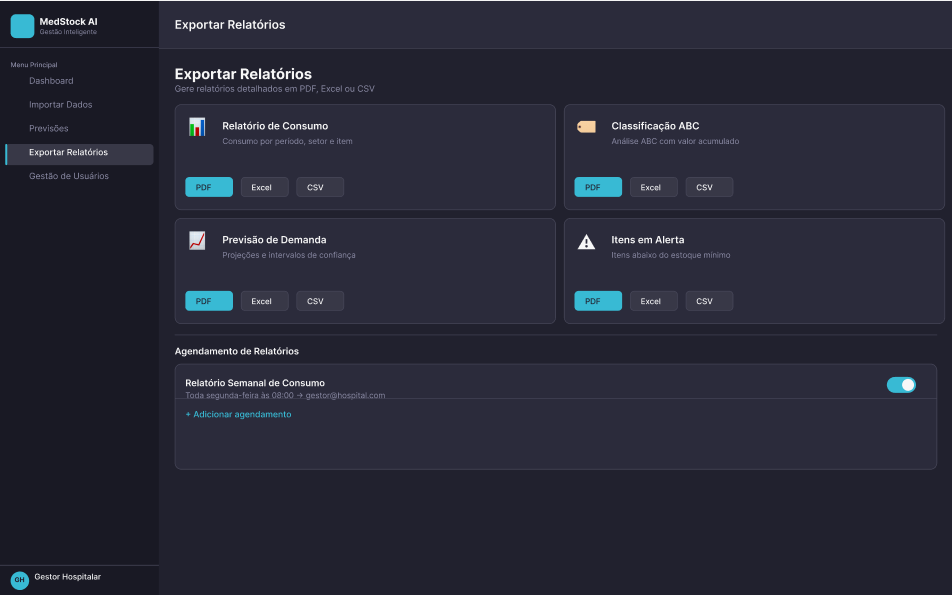
\includegraphics[width=0.8\textwidth]{Imagens/Mockups/Exportar_Relatorios.png}
    \caption{Tela de Exportar Relatório.}
\end{figure}

\paragraph{Gestão de Usuários}
Tela destinada ao cadastro de usuários, onde é definido o nível de acesso de cada um. O perfil Usuário tem acesso às telas Dashboard, Previsões e Exportar Relatório. O perfil Administrador possui acesso completo às funcionalidades da empresa. O perfil Super Admin é configurado via ambiente e possui acesso
irrestrito à plataforma, incluindo a Gestão de Empresas.

\textit{Ações principais:} cadastrar, editar e inativar usuários e definir perfil de acesso.

\begin{figure}[H]
    \centering
    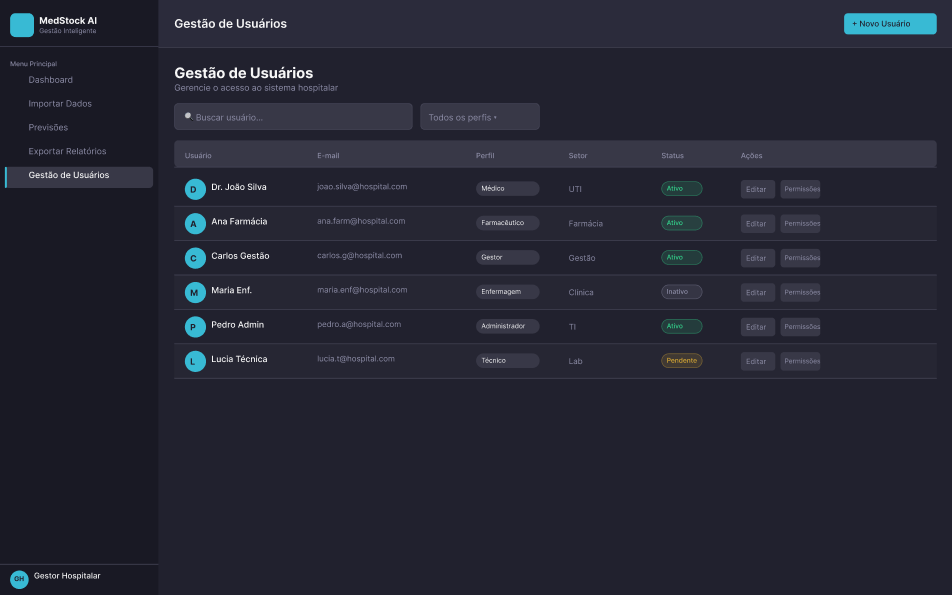
\includegraphics[width=0.8\textwidth]{Imagens/Mockups/Gestao_Usuarios.png}
    \caption{Tela de Gestão de Usuários.}
\end{figure}

\paragraph{Gestão de Hospitais}
Tela exclusiva do Super Usuário. Apresenta um painel com quatro indicadores no topo: total de instituições ativas, pendentes, inativas e o total geral cadastrado na plataforma. Abaixo, uma tabela lista todas as instituições com as colunas Responsável, E-mail, Hospital, Status e Ações. O filtro \textit{Todos os status} permite segmentar a listagem por situação. Para registros com status \textbf{Ativo} ou \textbf{Inativo}, a ação disponível é \textbf{Editar}. Para registros com status \textbf{Pendente}, os botões \textbf{Aprovar} e \textbf{Reprovar} substituem o Editar, permitindo ao Super Usuário analisar e deliberar sobre cada solicitação de acesso.

\textit{Ações principais:} visualizar indicadores de instituições, buscar hospital, filtrar por status, editar instituições ativas ou inativas e aprovar ou reprovar solicitações pendentes.

\begin{figure}[H]
    \centering
    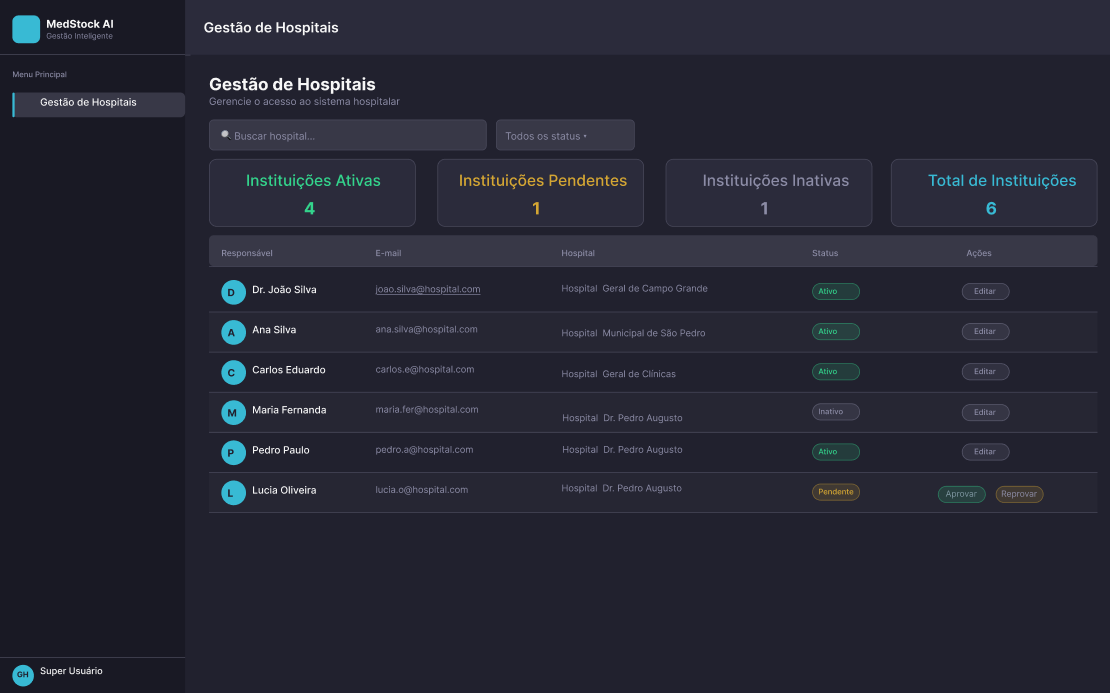
\includegraphics[width=0.8\textwidth]{Imagens/Mockups/Gestao_Hospitais.png}
    \caption{Tela de Gestão de Hospitais — Super Usuário.}
    \label{fig:gestao-hospitais}
\end{figure}

\paragraph{Solicitação de Acesso}
Tela pública acessível a partir da tela de Login, destinada a instituições interessadas em utilizar a plataforma. O formulário solicita três informações: Responsável pelo Contato, E-mail e Nome da Instituição. Após o envio, a solicitação é registrada no sistema com status \textbf{Pendente} e fica disponível para análise na tela de Gestão de Hospitais do Super Usuário.

\textit{Ações principais:} preencher dados da instituição e enviar solicitação de acesso.

\begin{figure}[H]
    \centering
    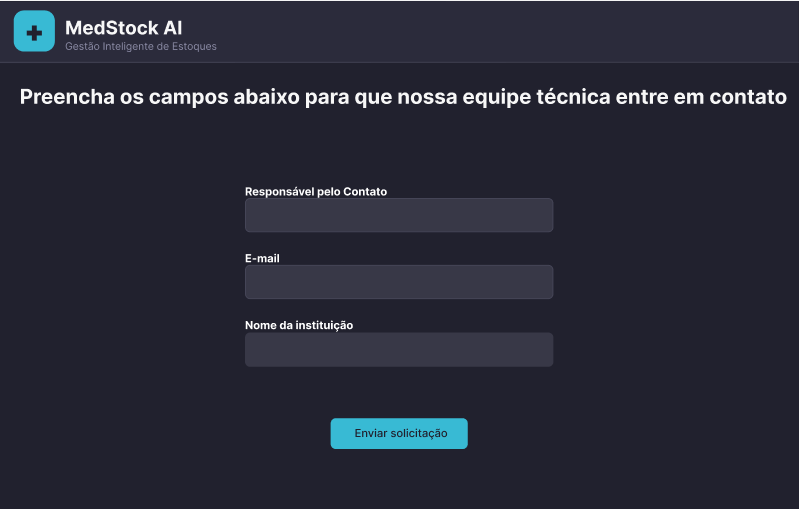
\includegraphics[width=0.8\textwidth]{Imagens/Mockups/Solicitacao_Acesso.png}
    \caption{Tela de Solicitação de Acesso.}
    \label{fig:solicitacao-acesso}
\end{figure}

\subsection{Fluxo de Interação do Usuário}

Serão apresentados dois fluxos de interação: o do Administrador e o do Usuário.

\vspace{0.4cm}
\noindent\textbf{Ator:} Administrador \\
\textbf{Objetivo:} Realizar a importação dos dados para o sistema e visualizar o Dashboard.

\begin{enumerate}
    \item Administrador acessa o sistema e realiza login com suas credenciais.
    \item O sistema valida as credenciais e redireciona para o Dashboard.
    \item O Dashboard exibe mensagem informando que não há dados importados.
    \item Administrador navega até a tela Importar Dados.
    \item Administrador seleciona o arquivo CSV com o histórico de consumo.
    \item O sistema realiza as validações automáticas dos dados.
    \item Importação concluída — o sistema confirma e registra no histórico.
    \item Administrador retorna ao Dashboard, que agora exibe KPIs e gráficos.
    \item Administrador analisa o consumo mensal e a classificação ABC dos itens.
\end{enumerate}

\vspace{0.4cm}
\noindent\textbf{Ator:} Usuário \\
\textbf{Objetivo:} Consultar previsão de demanda.

\begin{enumerate}
    \item Usuário acessa o sistema e realiza login com suas credenciais.
    \item O sistema valida as credenciais e redireciona para o Dashboard.
    \item O Dashboard exibe os KPIs e gráficos de consumo.
    \item Usuário navega até a tela Previsões.
    \item Usuário analisa quais itens terão maior consumo no período previsto.
\end{enumerate}

\vspace{0.4cm}
\noindent\textbf{Ator:} Super Usuário \\
\textbf{Objetivo:} Analisar e aprovar uma solicitação de acesso de novo hospital.

\begin{enumerate}
    \item Super Usuário acessa o sistema e realiza login com suas credenciais.
    \item O sistema valida as credenciais e redireciona para a tela de Gestão de Hospitais.
    \item Super Usuário visualiza os indicadores no topo da tela e identifica instituições com status Pendente.
    \item Super Usuário localiza a solicitação na tabela e analisa os dados da instituição.
    \item Super Usuário clica em \textbf{Aprovar} — o sistema atualiza o status da instituição para Ativo e os indicadores são atualizados.
\end{enumerate}

% -------------------------------------------------
\section{Arquitetura do Sistema}

\subsection{Diagrama C4}

\subsubsection{Nível 1: Diagrama de Contexto}

O diagrama de contexto apresenta o sistema como uma caixa preta, evidenciando
os atores que interagem com ele e os sistemas externos envolvidos. O perfil
Usuário consulta previsões e exporta relatórios, enquanto o Administrador
gerencia dados e usuários. O sistema consome dados históricos de um sistema
hospitalar externo (ERP/legado) via API REST ou arquivo CSV.

\begin{figure}[H]
    \centering
    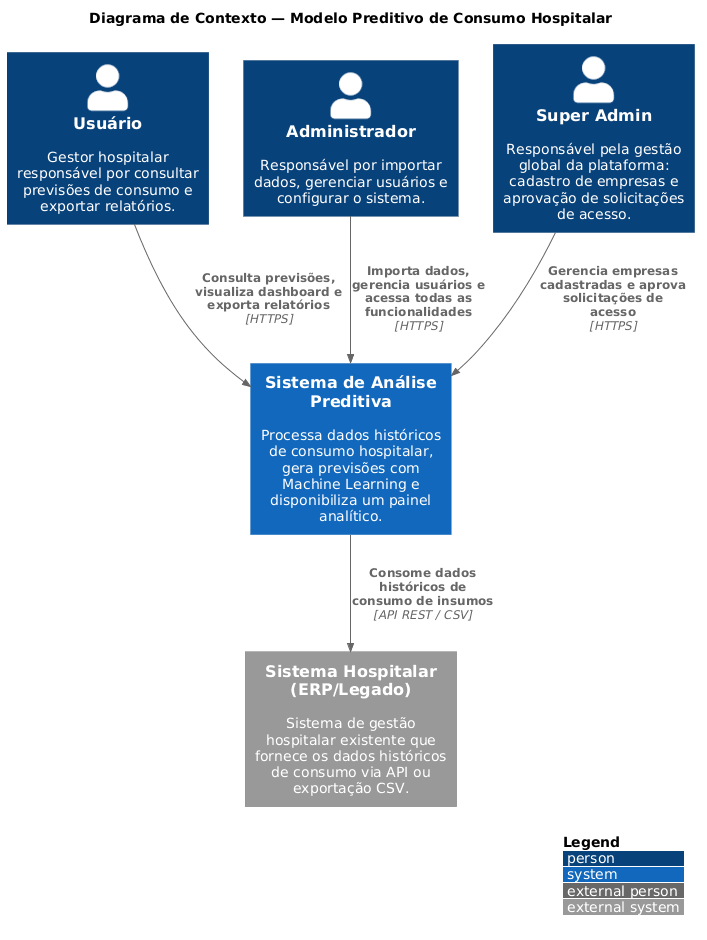
\includegraphics[width=0.75\textwidth]{Imagens/c4/C4_Contexto.png}
    \caption{Diagrama de Contexto C4 — visão macro do sistema e suas interações externas.}
    \label{fig:c4-contexto}
\end{figure}

\subsubsection{Nível 2: Diagrama de Containers}

O diagrama de containers decompõe o sistema em suas unidades de execução
independentes. A aplicação web (React/Next.js) comunica-se com a API REST
(FastAPI) via HTTPS. A API orquestra o Serviço de ML (LightGBM/Skforecast/Statsmodels)
e persiste os dados no banco PostgreSQL via SQLAlchemy. Adicionalmente, o
Job de Sincronização de Feriados (APScheduler) realiza uma consulta anual à
API externa \textit{feriados.dev}, que fornece feriados nacionais, estaduais
e municipais, e persiste os dados em uma tabela dedicada no banco PostgreSQL.
Dessa forma, o Serviço de ML consome os feriados diretamente do banco de dados
durante a engenharia de atributos do modelo preditivo, eliminando a dependência
de chamadas externas em tempo de inferência.

\begin{figure}[H]
    \centering
    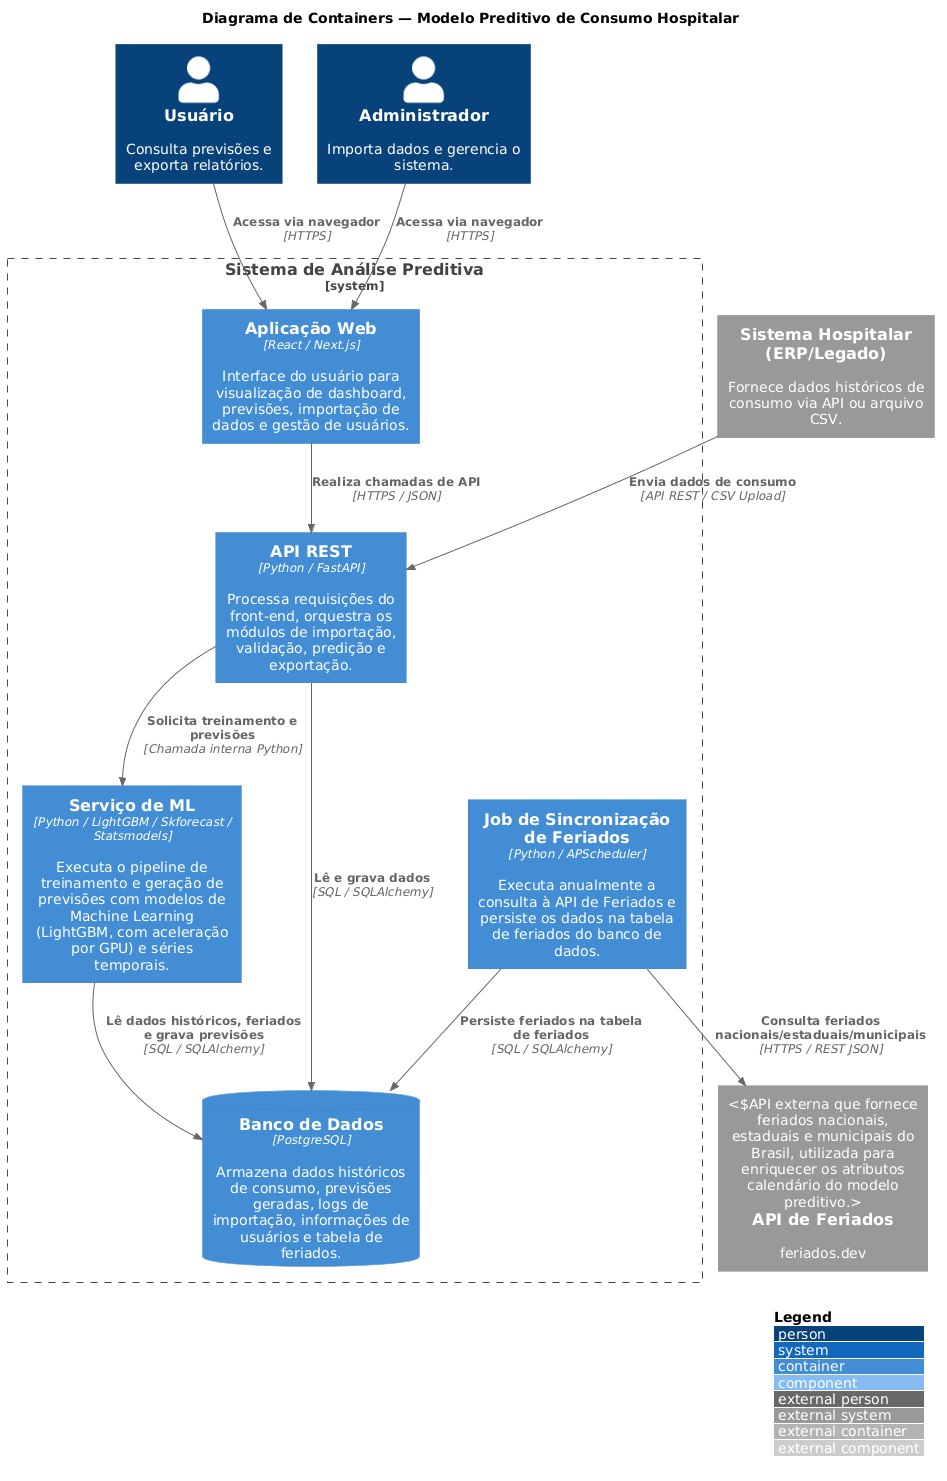
\includegraphics[width=0.65\textwidth]{Imagens/c4/C4_Containers.png}
    \caption{Diagrama de Containers C4 — arquitetura de alto nível e decisões tecnológicas.}
    \label{fig:c4-containers}
\end{figure}

\subsubsection{Nível 3: Diagrama de Componentes}

O diagrama de componentes detalha a estrutura interna da API REST, principal
container do sistema. São oito módulos com responsabilidades distintas:
Autenticação, Gestão de Usuários, Importação, Validação e Tratamento,
Previsão, Dashboard, Exportação de Relatórios e Sincronização de Feriados.
O Módulo de Previsão aciona o Serviço de ML, que consome os dados de
feriados diretamente do banco de dados durante a etapa de engenharia de
atributos. A consulta à API externa \textit{feriados.dev} é de
responsabilidade exclusiva do Módulo de Sincronização de Feriados, que
realiza essa operação uma vez ao ano e persiste os dados em uma tabela
dedicada no PostgreSQL.

\begin{figure}[H]
    \centering
    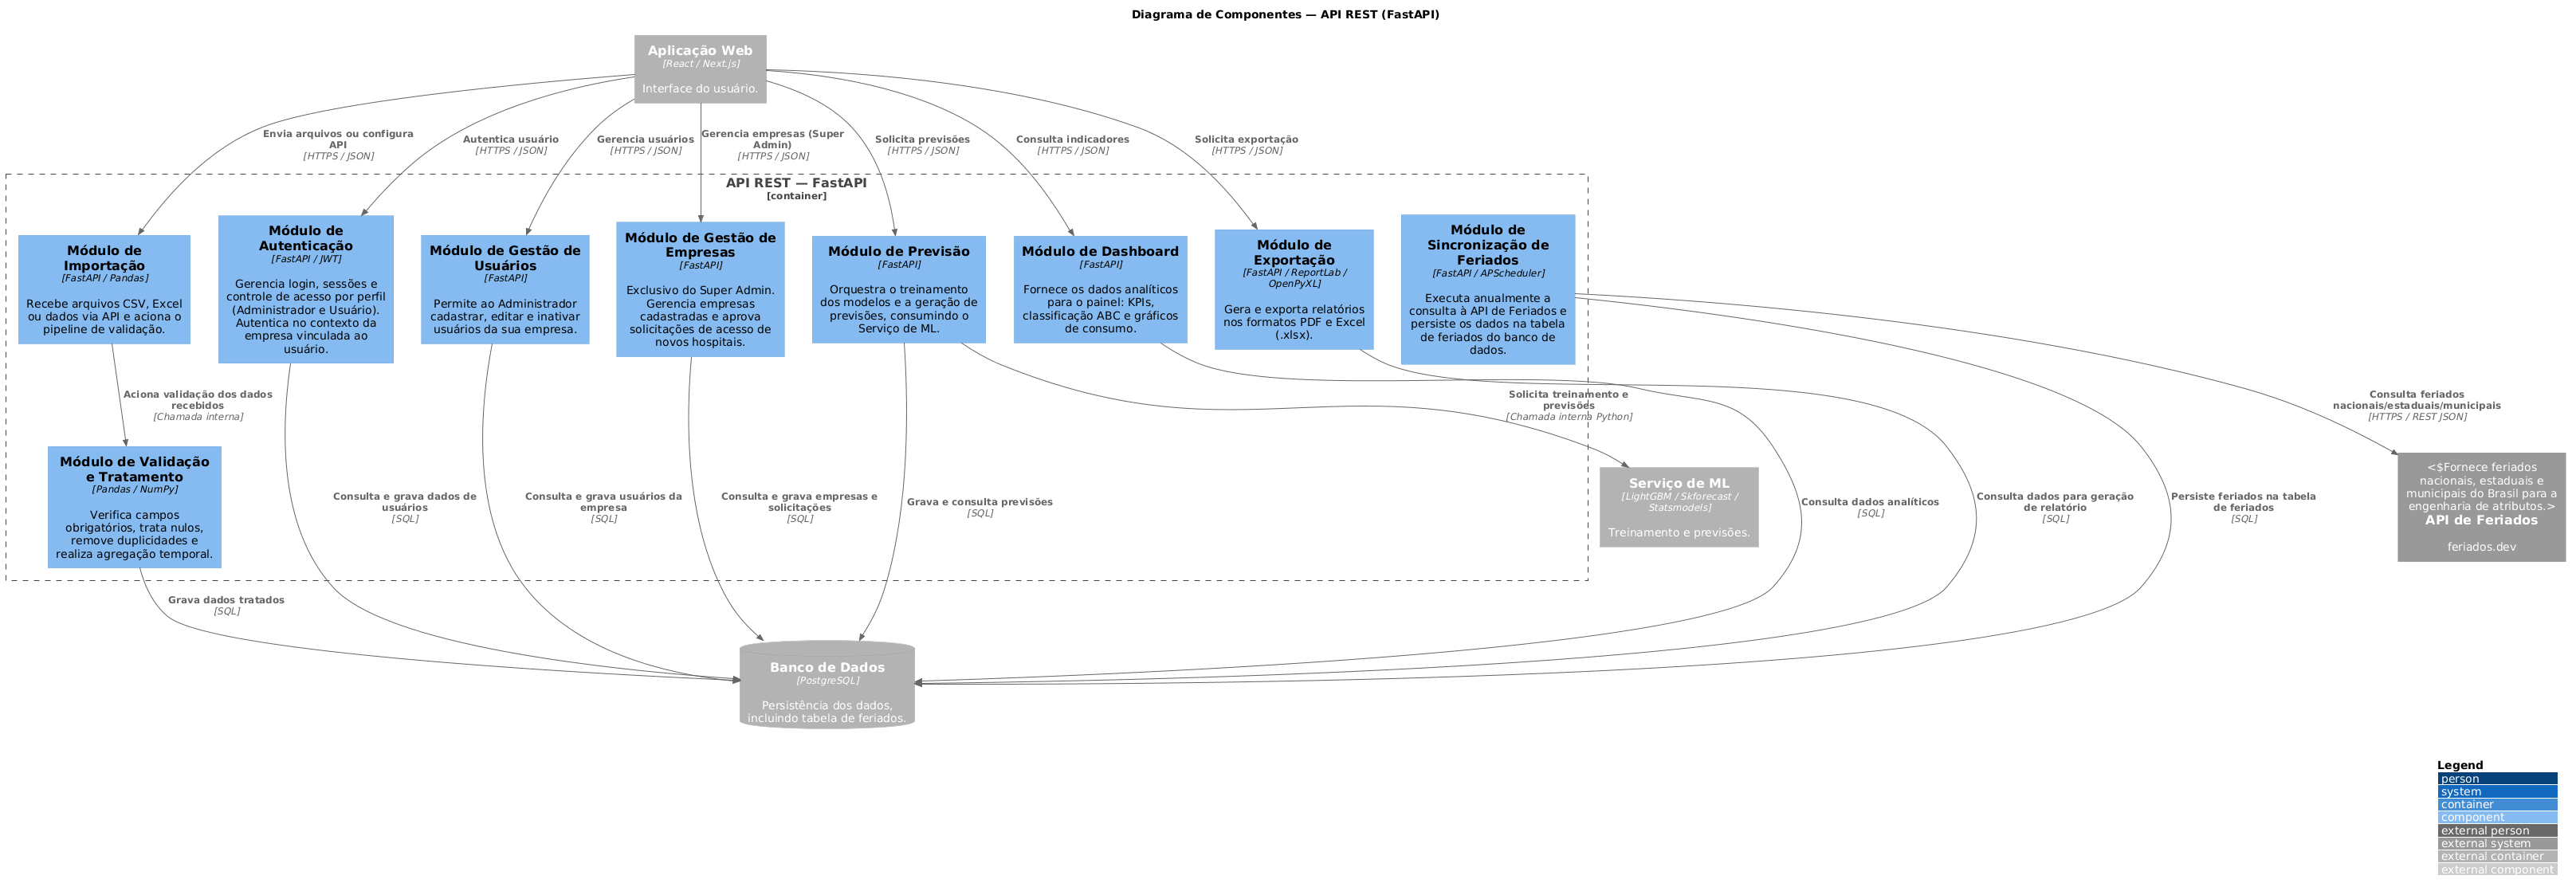
\includegraphics[width=1.10\textwidth]{Imagens/c4/C4_Componentes.png}
    \caption{Diagrama de Componentes C4 — estrutura interna da API REST (FastAPI).}
    \label{fig:c4-componentes}
\end{figure}

\FloatBarrier
\subsection{Modelo de Dados}

O sistema utiliza um banco de dados relacional PostgreSQL, organizado em
11 tabelas. Todas as tabelas de dados operacionais possuem o campo
\texttt{empresa\_id} para garantir o isolamento completo entre as
empresas cadastradas na plataforma.

\begin{figure}[H]
    \centering
    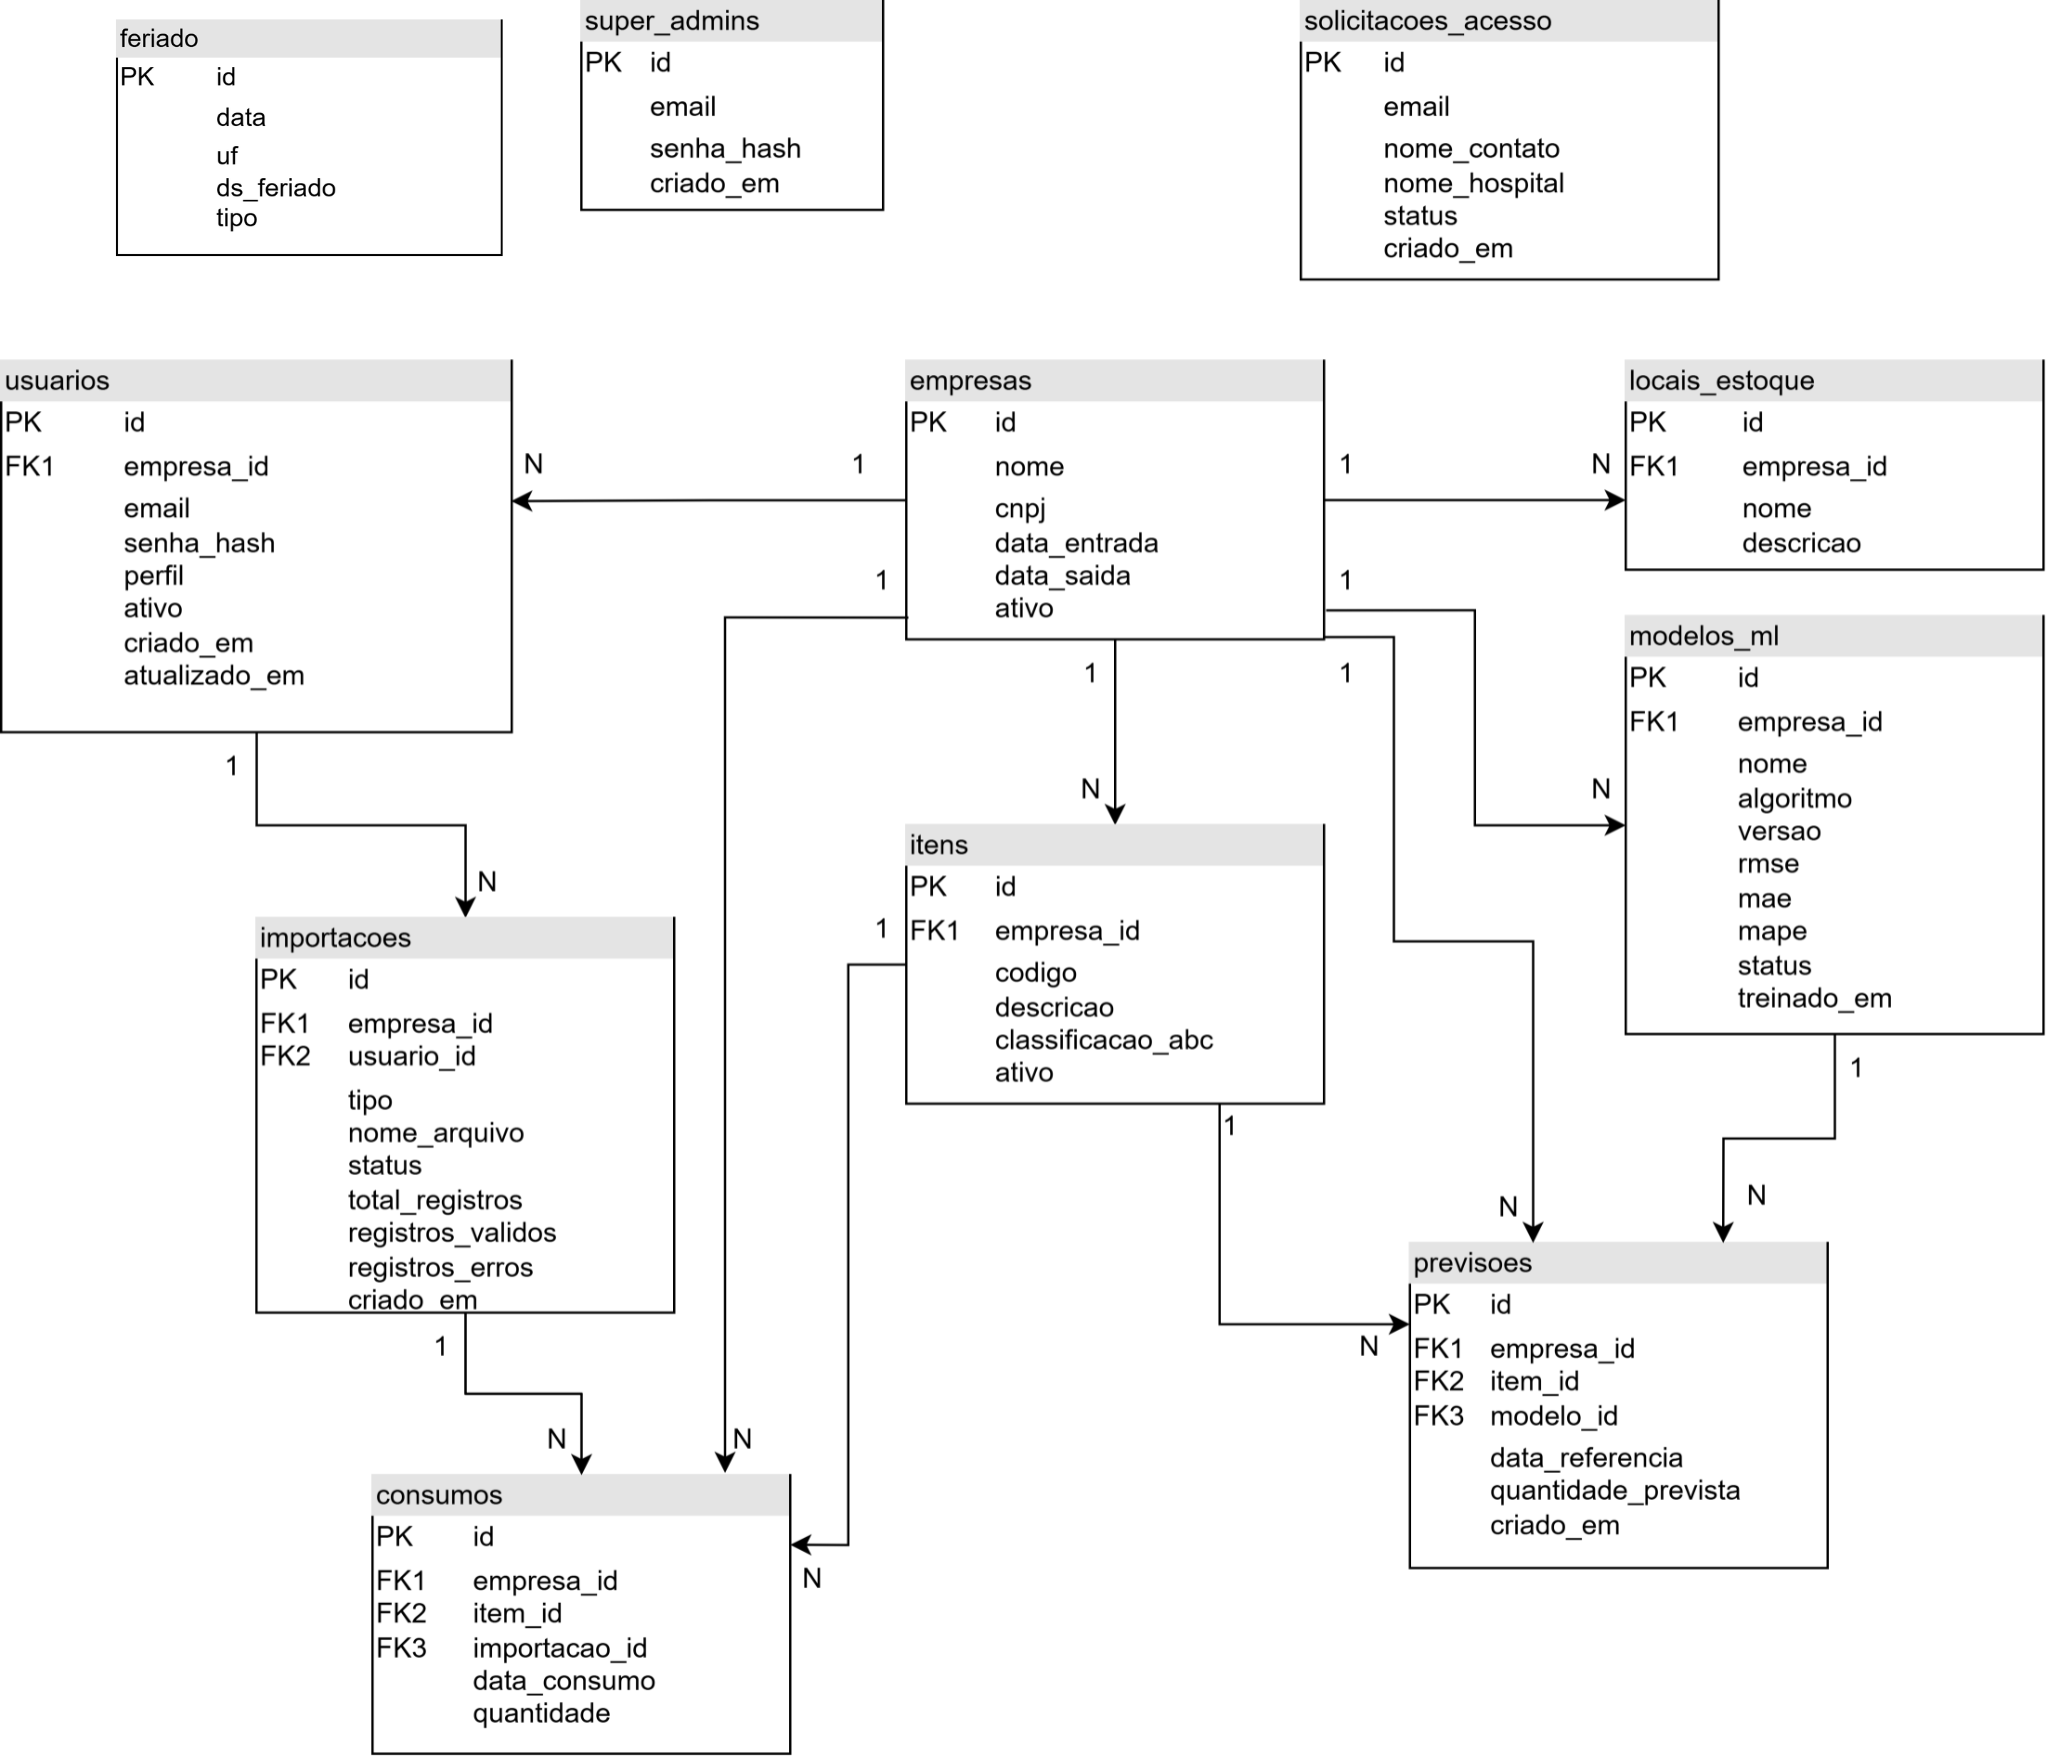
\includegraphics[width=1.10\textwidth]{Imagens/diagramas/TCC-DER.png}
    \caption{Diagrama de Entidade-Relacionamento — estrutura de tabelas.}
    \label{fig:Entidade-Relacionamento}
\end{figure}

\subsection{Principais Componentes}

O sistema é organizado em módulos com responsabilidades bem definidas,
descritos a seguir.

\paragraph{Módulo de Autenticação e Controle de Acesso:}
Responsável pelo gerenciamento de sessões e autenticação de usuários via JWT. Controla o acesso às funcionalidades do sistema de acordo com o perfil do usuário autenticado (Administrador ou Usuário), garantindo que apenas operações permitidas sejam executadas por cada perfil. Toda autenticação é realizada no contexto da empresa vinculada ao usuário, assegurando o isolamento de dados entre as organizações cadastradas na plataforma.

\paragraph{Módulo de Importação de Dados:}
Gerencia a entrada de dados históricos de consumo hospitalar na plataforma,
suportando upload manual de arquivos CSV e Excel, bem como integração via
API com periodicidade de carga configurável. Registra um histórico de todas
as importações realizadas.

\paragraph{Módulo de Validação e Tratamento de Dados:}
Executa o pipeline de qualidade sobre os dados recebidos, realizando
verificações de campos obrigatórios, tratamento de valores nulos, remoção
de duplicidades, validação de formatos de data e tipos de dados, além da
agregação temporal necessária para análise e predição.

\paragraph{Módulo de Treinamento e Predição:}
Núcleo analítico do sistema. Responsável pela execução do pipeline de
Machine Learning, contemplando a seleção e preparação de variáveis,
engenharia de atributos, separação de dados em treino e teste, treinamento
dos modelos (LightGBM, Skforecast e Statsmodels), avaliação por métricas (RMSE,
MAE e MAPE) e geração das previsões de consumo futuro.

\paragraph{Módulo de Visualização — Dashboard:}
Apresenta ao usuário os principais indicadores do sistema por meio de KPIs,
gráficos de consumo mensal, consumo por local de estoque, classificação ABC
dos itens e previsões de demanda. Consome os dados processados e as
previsões geradas pelo módulo de predição.

\paragraph{Módulo de Exportação de Relatórios:}
Permite a geração e exportação de relatórios consolidados nos formatos PDF
e Excel (.xlsx), disponível para todos os perfis de usuário.

\paragraph{Módulo de Gestão de Usuários:}
Permite ao Administrador cadastrar, editar e inativar usuários vinculados à sua empresa. Cada usuário recebe um perfil de acesso (Administrador ou Usuário) que determina as operações disponíveis no sistema. O isolamento entre empresas é garantido de forma que nenhum usuário consiga visualizar ou interagir com dados de outra organização.

\paragraph{Módulo de Gestão de Empresas (Super Admin):}
Componente exclusivo da conta de superadministrador da plataforma. Permite visualizar, ativar e inativar as empresas cadastradas, além de analisar e aprovar ou reprovar solicitações de acesso enviadas por novos hospitais interessados na plataforma. O acesso a este módulo é restrito ao superadministrador, cujas credenciais são configuradas por variáveis de ambiente no servidor, sem exposição na interface pública da aplicação.

\paragraph{API REST:}
Camada de comunicação entre o front-end e o back-end, implementada com
FastAPI. Expõe os endpoints necessários para autenticação, importação de
dados, consulta de previsões e exportação de relatórios, com documentação
gerada automaticamente.

\paragraph{Camada de Persistência:}
Responsável pelo armazenamento dos dados históricos, resultados de
previsões, logs de importação e informações de usuários. Implementada com
PostgreSQL como banco de dados relacional e SQLAlchemy como ORM para
comunicação com a aplicação Python.

\subsection{Stack Tecnológica}

\noindent{\textbf{Front-end}}
\begin{itemize}
    \item \textbf{Node.js:} Ambiente de execução JavaScript utilizado no front-end, escolhido pela ampla adoção e suporte a ferramentas modernas de desenvolvimento web.
    \item \textbf{React:} Biblioteca utilizada para construção da interface do usuário, permitindo o desenvolvimento de interfaces dinâmicas e reutilizáveis.
    \item \textbf{Next.js:} Framework baseado em React utilizado para estruturar a aplicação, oferecendo melhor organização, roteamento e otimização de performance.
\end{itemize}

\noindent{\textbf{Back-end}}
\begin{itemize}
    \item \textbf{FastAPI:} Framework web utilizado para construção da API do sistema, escolhido pela alta performance, suporte à tipagem com Python moderno e geração automática de documentação.
\end{itemize}

\noindent{\textbf{Dados/ML}}
\begin{itemize}
    \item \textbf{Pandas:} Biblioteca utilizada para manipulação e análise de dados tabulares, permitindo o tratamento e organização dos dados históricos de consumo.
    \item \textbf{NumPy:} Utilizado como base para operações numéricas, incluindo o cálculo das métricas de avaliação dos modelos (RMSE, MAE e MAPE).
    \item \textbf{Statsmodels:} Utilizada para aplicação de modelos de séries temporais, como SARIMA e Holt-Winters, voltados à previsão de consumo.
    \item \textbf{LightGBM:} Biblioteca de Gradient Boosting com suporte a treinamento acelerado por GPU, utilizada como principal motor de Machine Learning do projeto. Suporta nativamente variáveis categóricas (classificação ABC, local de estoque) e também permite treinar modelos no modo Random Forest.
    \item \textbf{Skforecast:} Framework que automatiza a geração de atributos de defasagem (lags) e janelas móveis, a previsão multi-step recursiva e a validação walk-forward sobre os modelos de Machine Learning.
\end{itemize}

\noindent{\textbf{Banco}}
\begin{itemize}
    \item \textbf{PostgreSQL:} Sistema de banco de dados relacional utilizado para armazenamento dos dados históricos e resultados das previsões.
    \item \textbf{SQLAlchemy:} Ferramenta ORM utilizada para facilitar a comunicação entre a aplicação em Python e o banco de dados.
\end{itemize}

\noindent{\textbf{API Externa}}
\begin{itemize}
    \item \textbf{feriados.dev:} API que fornece informações sobre feriados brasileiros, utilizada para incorporar impactos de datas comemorativas nas previsões de consumo. Disponiel em https://feriados.dev/
\end{itemize}

\subsection{Modelos Preditivos Utilizados}

\subsubsection{Critérios de Seleção}

A escolha dos modelos considerou as características do problema:
séries temporais de consumo hospitalar com possível presença de
sazonalidade, tendência e outliers decorrentes de eventos pontuais
(surtos, campanhas de vacinação, etc.). Os critérios utilizados foram:

\begin{itemize}
    \item \textbf{Adequação ao tipo de dado:} capacidade de lidar com
          séries temporais irregulares e com diferentes volumes de histórico por
          item;
    \item \textbf{Interpretabilidade:} modelos cujos resultados possam ser
          compreendidos por gestores sem formação técnica em ciência de dados;
    \item \textbf{Compatibilidade com a stack definida:} modelos disponíveis
          nas bibliotecas LightGBM, Skforecast e Statsmodels, já previstas na arquitetura;
    \item \textbf{Diversidade de abordagem:} combinar modelos estatísticos
          clássicos de séries temporais com modelos de Machine Learning, permitindo
          comparação entre paradigmas.
\end{itemize}

\subsubsection{Modelos Candidatos}

\begin{longtable}{p{0.22\textwidth} p{0.22\textwidth} p{0.45\textwidth}}
    \toprule
    \textbf{Modelo}                                       & \textbf{Categoria} & \textbf{Descrição e Justificativa} \\
    \midrule
    \endfirsthead
    \toprule
    \textbf{Modelo}                                       & \textbf{Categoria} & \textbf{Descrição e Justificativa} \\
    \midrule
    \endhead

    Média Móvel Simples (SMA)                             &
    Baseline                                              &
    Calcula a média aritmética das últimas $n$ observações como previsão para
    o período seguinte. Utilizado exclusivamente como \textit{baseline} de
    referência: qualquer modelo candidato deve superar esse resultado para ser
    considerado.                                                                                                    \\
    \midrule

    SARIMA \newline (Seasonal ARIMA)                      &
    Séries Temporais Clássico                             &
    Extensão do ARIMA com componente sazonal explícito $(p,d,q)(P,D,Q)_s$.
    Indicado para séries com tendência e sazonalidade periódica, como o consumo
    de determinados medicamentos com padrão mensal ou sazonal.
    Implementado via \texttt{statsmodels.tsa.statespace.SARIMAX}.                                                   \\
    \midrule

    Holt-Winters \newline (Suavização Exponencial Tripla) &
    Séries Temporais Clássico                             &
    Modelo aditivo ou multiplicativo que decompõe a série em nível, tendência
    e sazonalidade, atribuindo pesos exponencialmente decrescentes às
    observações mais antigas. Robusto para séries curtas e com sazonalidade
    estável. Implementado via \texttt{statsmodels.tsa.holtwinters.ExponentialSmoothing}.                            \\
    \midrule

    Random Forest \newline (modo LightGBM)                &
    Machine Learning                                      &
    Ensemble de árvores de decisão do LightGBM, com aceleração por GPU,
    sobre variáveis derivadas da série temporal (lags, médias móveis,
    indicadores de mês, semana e dia da semana). Captura relações não
    lineares, é robusto a outliers e permite avaliar a importância de
    cada atributo, apoiando a interpretabilidade exigida pelo RNF03.
    Implementado via \texttt{lightgbm.LGBMRegressor}.                                                               \\
    \midrule

    Gradient Boosting \newline (LightGBM)                 &
    Machine Learning                                      &
    Método de boosting baseado em árvores de decisão sequenciais que minimiza
    o erro residual a cada iteração, com suporte nativo a variáveis
    categóricas e treinamento acelerado por GPU. Apresenta excelente
    desempenho em dados tabulares com engenharia de atributos temporal e
    é amplamente utilizado em competições de previsão de demanda em nível
    de item (ex.: M5), com potencial de maior acurácia em conjuntos de
    dados maiores e com maior heterogeneidade entre itens.
    Implementado via \texttt{lightgbm.LGBMRegressor}.                                                               \\

    \bottomrule
\end{longtable}

\subsubsection{Estratégia de Avaliação}

Todos os modelos serão avaliados sob a mesma estratégia de validação
temporal (\textit{walk-forward validation}), na qual o conjunto de treino
é expandido progressivamente e as previsões são realizadas sempre sobre
dados futuros não vistos pelo modelo. Essa abordagem evita o vazamento
de informação temporal (\textit{data leakage}), que ocorreria com uma
divisão aleatória dos dados.

\vspace{0.3cm}
\noindent As métricas utilizadas para comparação serão MAPE, MAE e RMSE,
calculadas via NumPy/Pandas (ou pelas funções de métrica nativas do
Skforecast), conforme definido nos KPIs do projeto (Seção~1.5). O modelo
com menor MAPE médio sobre os itens de maior criticidade (Classe A da
curva ABC)
será adotado como modelo principal em produção. Os demais permanecerão
disponíveis no pipeline para seleção automática por item, caso um modelo
alternativo apresente desempenho superior para determinado grupo de
insumos.

\subsubsection{Engenharia de Atributos}

Para os modelos de Machine Learning (Random Forest e Gradient Boosting),
serão construídas as seguintes variáveis derivadas a partir da série
histórica de consumo:

\begin{itemize}
    \item \textbf{Lags temporais:} consumo dos períodos anteriores
          ($t-1$, $t-2$, $t-3$, $t-6$, $t-12$);
    \item \textbf{Médias móveis:} médias de 3, 6 e 12 períodos anteriores;
    \item \textbf{Indicadores calendário:} mês do ano, trimestre,
          indicador de fim de ano e indicador de mês de alta sazonalidade;
    \item \textbf{Indicador de feriado:} flag booleana indicando se a
          data de referência corresponde a um feriado nacional, estadual
          ou municipal, obtida por meio da API externa
          \textit{feriados.dev};
    \item \textbf{Classificação ABC do item:} variável categórica
          indicando a criticidade do insumo;
    \item \textbf{Estoque local:} setor ou local de estoque ao qual o
          item pertence, quando disponível nos dados históricos.
\end{itemize}

\noindent{A integração com a API \textit{feriados.dev} é realizada pelo
    Serviço de ML durante a etapa de engenharia de atributos, consultando os
    feriados do período correspondente ao histórico de consumo e mapeando-os
    para a granularidade temporal utilizada pelo modelo (diária, semanal ou
    mensal).}

\noindent{A geração dos atributos de defasagem (lags) e médias móveis,
    bem como a previsão multi-step recursiva, são automatizadas por meio da
    biblioteca \textit{Skforecast}, que integra modelos como o LightGBM ao
    processo de validação walk-forward, seguindo a interface padrão de
    treinamento e predição (\texttt{fit}/\texttt{predict}).}

% -------------------------------------------------
\section{Segurança e Privacidade}
\subsection{Privacidade e LGPD}

O sistema foi projetado com foco na minimização de dados, processando
apenas as informações estritamente necessárias para a finalidade proposta.
Não são coletados, armazenados ou processados dados de pacientes ou
quaisquer informações de saúde de pessoas físicas, o que reduz
significativamente o escopo de exposição à Lei Geral de Proteção de Dados
(LGPD — Lei nº 13.709/2018).

\paragraph{Dados coletados}
O sistema opera com duas categorias de dados:

\begin{itemize}
    \item \textbf{Dados de consumo hospitalar:} código do item, descrição,
          data, quantidade de consumo e local de estoque. Trata-se de dados
          operacionais e institucionais, sem vínculo com pessoas físicas
          identificadas ou identificáveis.

    \item \textbf{Dados dos usuários do sistema:} nome, e-mail e perfil de
          acesso dos usuários cadastrados (Administrador e Usuário). Estes
          constituem dados pessoais nos termos da LGPD e estão sujeitos às
          obrigações da lei.
\end{itemize}

\paragraph{Armazenamento e segurança}
Os dados são armazenados em banco de dados relacional (PostgreSQL), com
acesso restrito a usuários autenticados. As senhas dos usuários são
armazenadas de forma criptografada, e a comunicação entre cliente e
servidor é realizada exclusivamente via HTTPS, conforme definido no RNF11.

\paragraph{Direitos dos titulares}
Em conformidade com a LGPD, os usuários cadastrados no sistema podem
solicitar ao Administrador:
\begin{itemize}
    \item acesso aos seus dados pessoais armazenados;
    \item correção de dados incompletos ou desatualizados;
    \item exclusão de seus dados, mediante inativação ou remoção do
          cadastro pelo Administrador.
\end{itemize}

% -------------------------------------------------
\section{Planejamento do Projeto}

O planejamento foi organizado em 5 marcos, descritos abaixo com suas respectivas datas previstas.

\begin{center}
    \begin{tabular}{p{0.10\textwidth} p{0.60\textwidth} p{0.20\textwidth}}
        \toprule
        \textbf{Marco} & \textbf{Descrição}                                                                                                        & \textbf{Prazo} \\
        \midrule
        M1             & Finalização da documentação RFC, contemplando levantamento de requisitos, arquitetura, mockups e planejamento do projeto. & 15/06/2026     \\
        \midrule
        M2             & Desenvolvimento do back-end, contemplando API REST, pipeline de importação e validação de dados, e camada de persistência & 16/08/2026     \\
        \midrule
        M3             & Desenvolvimento do front-end da aplicação, incluindo todas as telas definidas nos mockups e integração com a API.         & 05/10/2026     \\
        \midrule
        M4             & Integração dos módulos, testes finais do sistema e entrega da versão completa do projeto.                                 & 30/11/2026     \\
        \bottomrule
    \end{tabular}
\end{center}

% -------------------------------------------------
\section{Referências}

\begin{thebibliography}{99}

    \bibitem{aptel2001}
    APTEL, O.; POURJALALI, H. Improving activities and decreasing costs of logistics in
    hospitals: a comparison of U.S. and French hospitals. \textit{The International Journal
        of Health Planning and Management}, v.~16, n.~6, p.~413--426, 2001.

    \bibitem{barbieri2006}
    BARBIERI, J. C.; MACHLINE, C. \textit{Logística hospitalar: teoria e prática}.
    São Paulo: Saraiva, 2006.

    \bibitem{slimstock2024}
    SLIMSTOCK. \textit{Software de Previsão de Demanda}. Disponível em:
    \url{https://www.slimstock.com/pt/solucoes/software-previsao-demanda/}.
    Acesso em: abr. 2026.

    \bibitem{o9solutions2024}
    O9 SOLUTIONS. \textit{AI/ML Forecasting --- Demand Planning}. Disponível em:
    \url{https://o9solutions.com/solutions/demand-planning/ai-ml-forecasting}.
    Acesso em: abr. 2026.

    \bibitem{gtplan2024}
    GTPLAN. \textit{Gestão de Estoque Hospitalar}. Disponível em:
    \url{https://gtplan.net/}. Acesso em: abr. 2026.

    \bibitem{bionexo2024}
    BIONEXO. \textit{Plataforma de Gestão Hospitalar}. Disponível em:
    \url{https://bionexo.com/}. Acesso em: abr. 2026.

\end{thebibliography}

\section{Apêndices}

\subsection{Protótipo de Interface}
O protótipo de alta fidelidade do sistema foi desenvolvido na ferramenta
Figma, contemplando todas as telas descritas na seção 4 deste documento.
O protótipo pode ser acessado pelo link a seguir:
\begin{center}
    \url{https://www.figma.com/design/AhP2PCySRYgYfjRPKHZRTY}
\end{center}

\subsection{Diagramas e Casos de Uso}
Os diagramas de casos de uso e o fluxo de navegação apresentados nesta
documentação foram desenvolvidos na ferramenta draw.io. Os arquivos podem
ser acessados pelo link a seguir:
\begin{center}
    \url{https://app.diagrams.net/?src=about#G11MZcrJfoFZt-voZ4wql40aV1GSZYBvYj#%7B%22pageId%22%3A%225-c5bP9vLpfaQluYnJfG%22%7D}
\end{center}

\subsection{Diagramas C4 — Código-Fonte}
Os diagramas C4 apresentados na seção 5.1 foram gerados com a linguagem
PlantUML utilizando a biblioteca C4-PlantUML. Os códigos-fonte estão
disponíveis no repositório do projeto e podem ser reproduzidos em qualquer
ambiente com suporte a PlantUML.

\subsection{Repositório do Projeto}
O código-fonte do sistema será disponibilizado publicamente ao final do
desenvolvimento no repositório a seguir:
\begin{center}
    \url{https://github.com/Luizmichels/MedStock-AI}
\end{center}

\newpage
\section{Assinatura do Comitê de Avaliação}

\vspace{3cm}
\noindent\rule{\textwidth}{0.1pt}
\centerline{Prof. Claudinei Dias}

\vspace{3cm}
\noindent\rule{\textwidth}{0.1pt}
\centerline{Profa. Janaina Fontana Biffi Duarte}

\end{document}
